%!TEX root = ../PhDthesis.tex
\chapter{A spatially calibrated model of visual cortex}

One of the major obstacles in modern neuroscience is integrating the
vast amount of experimental data that has been generated, highlighting
where different sources of evidence is and is not in agreement and
offering testable hypothesis to resolve such discrepancies. The
primary visual cortex is one of the most well studied areas in the
mammalian brain and we have previously seen that it has been
extensively explored at varying levels of description, from
development, circuits and anatomy to surround modulation, behavioral
studies and theoretical models of computation.

In order to provide a better account on how all this information fits
together in a generalized model describing the organization and
computations performed by the cortex, a unified reference frame
regarding the various spatial scales is desperately needed. A careful
reading of the literature highlights just how dependent various
effects are on the spatial profiles of the underlying neurite
projections. Here I will present a developmental model that takes
these levels of evidence into account, allowing us to cross-validate
known anatomical properties by confirming them against the response
properties of the model after development. This will allow bridging
between known measurements of anatomy and circuitry and
electro-physiological or even behavioral experiments performed on
visual cortex.

So far only very few attempts have been made at developing models that
take into account the various spatial properties that have been
described in the literature ranging from anatomy to
electro-physiological measurements. This chapter will demonstrate how
existing models of cortical development, specifically the Gain Control
Adaptation Lateral model (GCAL) \citep{Stevens2013} can be calibrated
to match known measurements of spatial extents more closely in a new
\textbf{S}patially \textbf{CAL}ibrated (SCAL) model.

The analysis will focus on various experimental assessments of the
spatial properties of the visual pathway and describe how we can use
these to build a model that achieves a high-level of consistency with
experimental results across a wide range of measures. Specifically,
the model will be calibrated with experimental measurements in the
parafoveal regions of the visual system of macaque. The macaque has
long been a experimental model for in visual neuroscience and the
literature surrounding contextual modulation in particular. In doing
so this chapter will critically evaluate the literature surrounding
spatial tuning properties in the mammalian cortex, highlighting
discrepancies and specifically assessing various models used to
characterize the spatial tuning properties of neurons in the visual
pathway.

Once we have collected the data we will provide a full
characterization of the spatial response properties, receptive fields
and synaptic weights in the model confirming they closely match
experimental data. At the same time we will outline in which ways the
model falls short and discuss some ways in which these shortcomings
might be remedied, which we will pick up in the following chapters.
In particular we will highlight problems with the classical GCAL
architecture, which makes no distinction between excitatory and
inhibitory cell classes and how that relates to the spatial
calibration and long-range surround suppression, which is thought to
be mediated by disynaptic, long-range excitatory mechanisms.

\section{Methods}

In this chapter we first introduce the developmental models of the
primary visual cortex the more complex models are based on. We begin
by outlining the equations and mechanisms underpinning these models
and then describe various analyses we can apply to these models to
replicate experimental protocols and compare the model against
experimental results.

\subsection{A spatially calibrated model of cortical development} 

The GCAL model put forth in \cite{Stevens2013} will serve as the
starting point for the models in this thesis. As discussed previously
(see \ref{devmodels}), it provides the first model that develops
robust and stable orientation maps independent of visual contrast and
for a wide range of training inputs. In this section we describe the
equations governing this model, how it is structured and will
highlight the modifications that were made to achieve a more
consistent spatial calibration.

The major changes introduced in this model are the replacement of
subtractive with divisive inhibition and large changes to the spatial
profile of connections. One of the major issues we will attempt to
settle here is whether the formation of orientation maps requires real
long-range inhibitory connections or whether the extents of known
inhibitory cell classes is sufficient to account the development of
smooth and robust orientation maps. Additionally we add an optional
long-range excitatory connection to the model to determine if the
model develops in a realistic manner. Before analyzing the behavior of
the model we describe its overall architecture and the equations
governing its behavior.

\subsubsection{Architecture}

The architecture of this family of models builds on two main concepts,
the idea of 2D sheets of firing-rate point neurons and projections
between them, representing the synaptic connections between the
neurons. All models we will introduce share the same basic
organization at the retinal and lateral geniculate nucleus level, but
will introduce increasingly complex models of the interactions in the
primary visual cortex. In Figure \ref{LGNDiagram} you can see the
organization of the retinal and lateral geniculate nucleus ON and OFF
sheets.

\begin{figure}
	\centering
        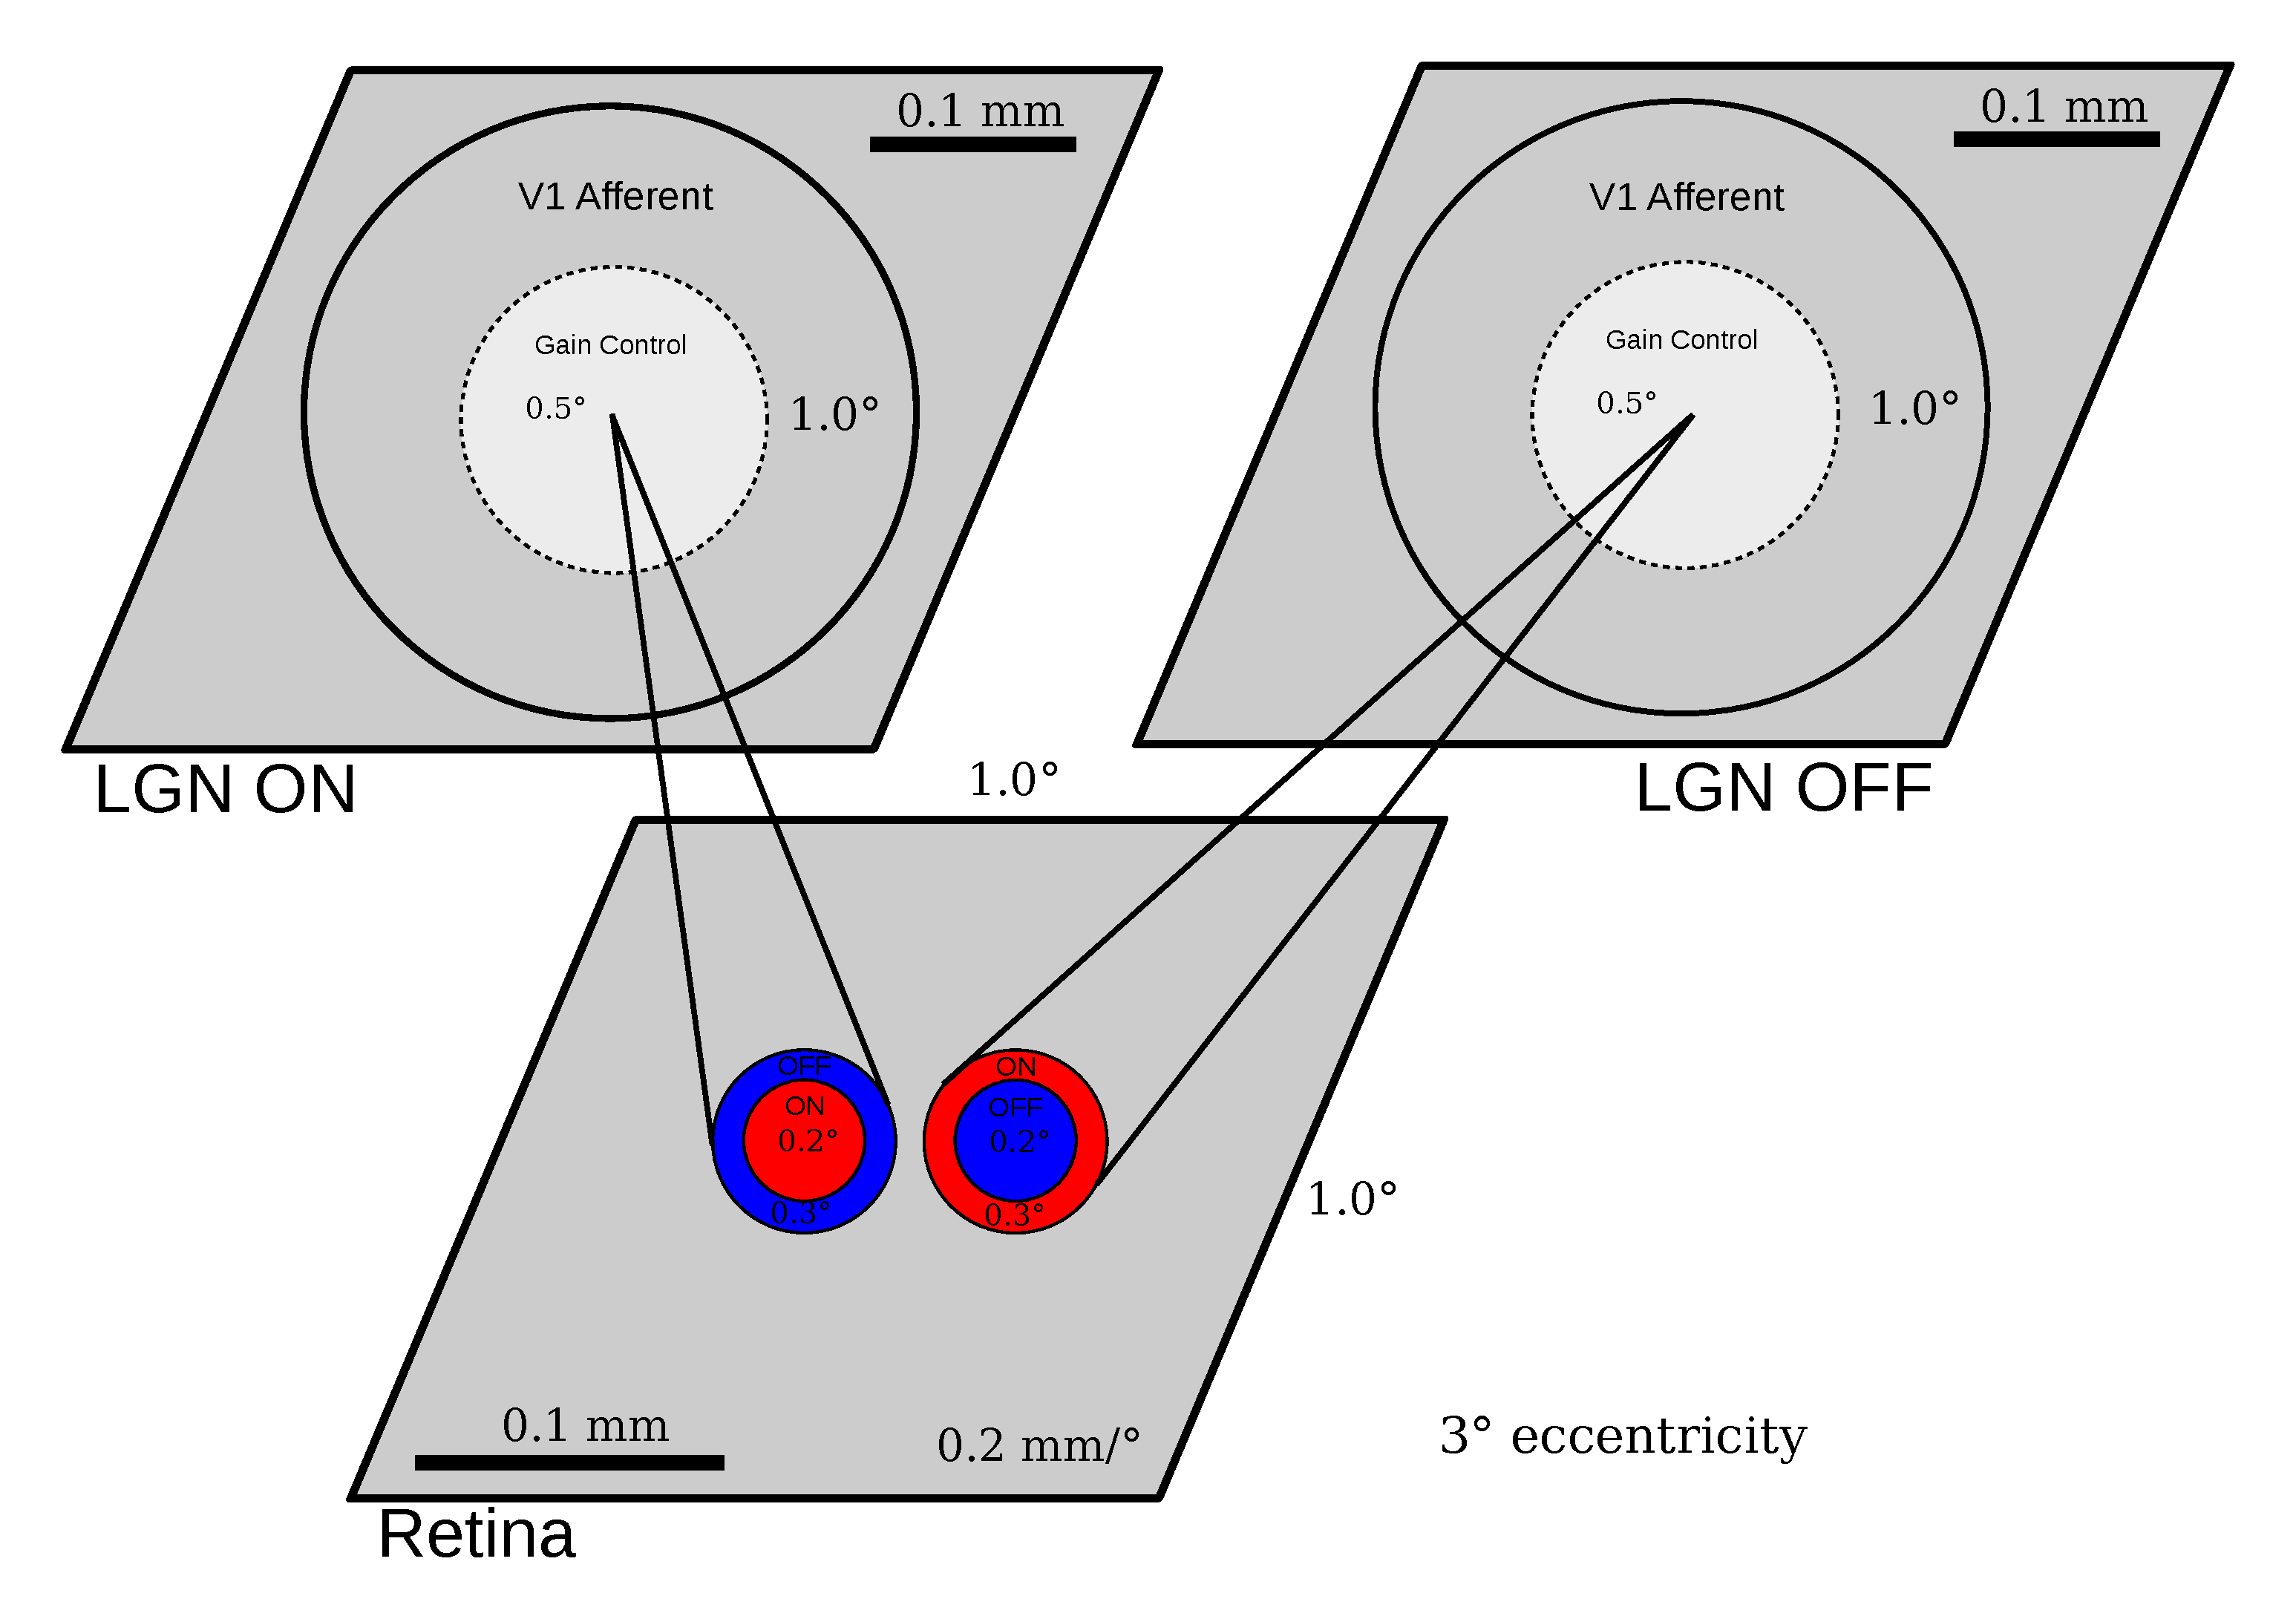
\includegraphics[width=1.0\textwidth]{LGN_Diagram.pdf}
	\caption[Diagram of the SCAL retinogeniculate stage.]{Diagram of
      the retinogeniculate stages of the spatially calibrated (SCAL)
      model. At the LGN level the excitatory and inhibitory
      center-surround components are shown in red and blue
      respectively. In the LGN the absolute size of the divisive gain
      control connection is indicated by a solid line while the
      diameter of the Gaussian used to initialize the lateral weights
      is marked by a dotted line. The given spatial scales hold for an
      eccentricity of 3\degree in macaque retina and LGN.}
	\label{LGNDiagram}
\end{figure}

The model operates by presenting patterns on the retinal sheet, which
then get filtered through difference-of-gaussian connection fields,
which give rise to the response the ON and OFF sheets. There a lateral
gain control projection applies some pooling normalization to the
response. This early stage of processing represents a crude model of
retinal ganglion and LGN function and provides the input to the
various cortical models introduced here.

The architecture of the retinal ganglion cell and lateral geniculate
nucleus layers will remain unchanged for all the models presented in
this thesis, while the V1 stage will be progressively refined.

The model diagram for the SCAL V1 stage is shown in \ref{SCALDiagram}
consisting of a single neural sheet with a comparatively large
afferent connection when considered against the GCAL model. The local
excitatory and inhibitory kernels however have changed only slightly
in their size and finally the model optionally includes a long-range
excitatory connection, which represents the long-range patchy lateral
connectivity that is so characteristic of layer 2/3 in the visual
cortex of higher mammals.

\begin{figure}
	\centering
        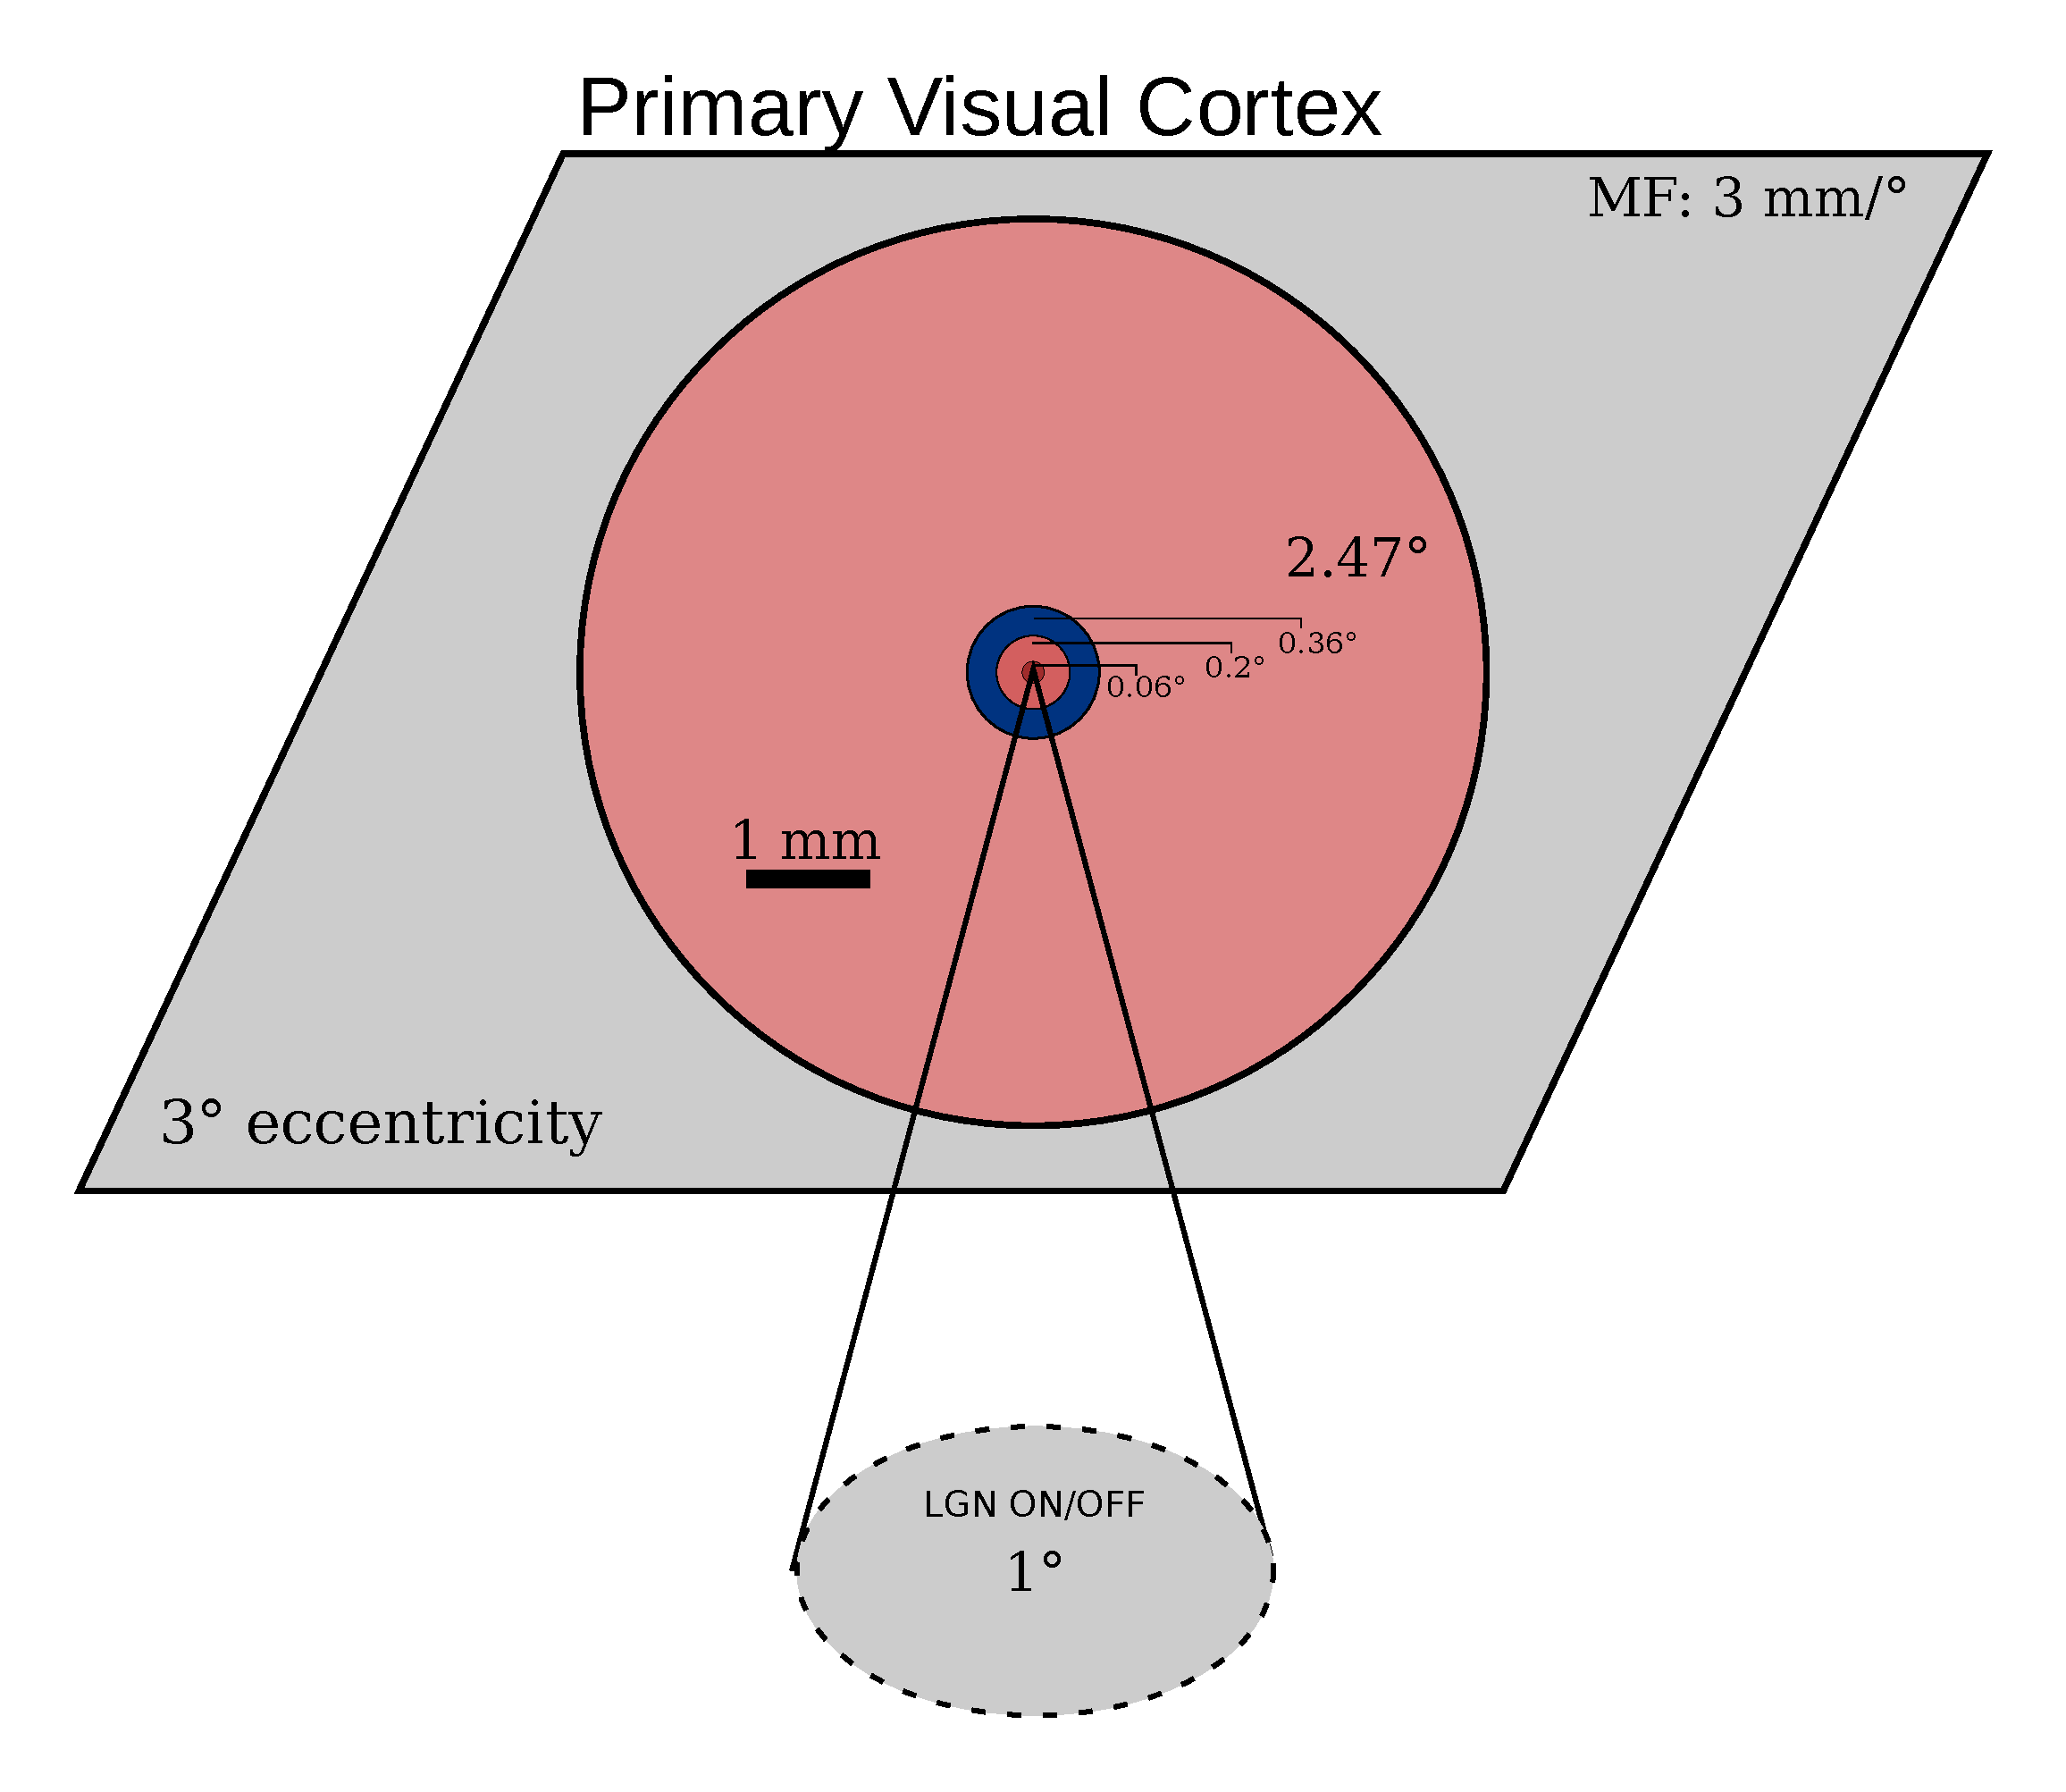
\includegraphics[width=1.0\textwidth]{SCAL_Diagram.pdf}
	\caption[Schematic representation of the SCAL model.]{Diagram of
      the SCAL V1 stage of the model showing the spatial scales of the
      various excitatory (red) and inhibitory (blue)
      connections. Saturated colors indicate the kernel radii, while
      lightly shaded regions indicate kernel cut-off extents.}
	\label{SCALDiagram}
\end{figure}

\subsubsection{Input patterns}

The organization of the self-organizing map (SOM) based developmental
models of the cortex, is determined by a complex interplay between the
model and the input patterns it is trained on. Just as in the
developing brain connections are formed depending on the statistics of
the sensory experience of the strongly influencing the spatial
organization of the model. In order to accurately assess how the
models respond to and self-organize in different visual environments
we will use three different visual stimuli to present to the model.

The simplest pattern used as the baseline for most measurements will
be simply elongated Gaussian patterns matching the length of the
integrative area of a V1 neuron and with a spatial frequency that
would allow three distinct lobes to form within this area. The
training patterns are given by:

\begin{equation}
  exp(-x^2/(2*\sigma_x^2) - y^2/(2*\sigma_y^2)
\label{eqn:gausspattern}
\end{equation}

Additionally two image datasets will be employed one taken from a
database of natural images and the other recorded from within the
rearing environment of ferrets in a laboratory, which is dominated by
the long co-linear statistics of the cage bars. These datasets will
allow us to explore the effect of the natural image statistics on the
organization of the models and confirm robustness against a wide range
of visual input.

\subsubsection{Activation}

All the models operate by presenting a new retinal input at each
iteration updating the activation of each unit in each sheet. The
neurons in the sheets are firing-rate point neurons, with the main
state being a floating point activation value.  For all models, the
activation level $\eta$ for a unit at position $j$ in an ON/OFF sheet
O at time $t+\delta t$ is defined as:

\begin{equation}
\eta_{j, O}(t+\delta t)=f\left(\frac{\gamma_{O}\sum_{i\in
    F_{j,P}}\Psi_{i}(t)\omega_{ij}}{k+\gamma_{S}\sum_{i\in
    F_{j,S}}\eta_{i, O}(t)\omega_{ij, S}}\right)
\label{eqn:lgnactivation}
\end{equation}

The constant $\gamma_{O}=14.0$ is an arbitrary multiplier for the
overall strength of connections from the photoreceptor sheet to the
ON/OFF sheets, chosen to give typical activations in the range 0.0 to
1.0, while $\gamma_{S}$ is the strength of the feed-forward
contrast-gain control. $\Psi_{i}$ is the activation of unit $i$ in the
two-dimensional array of neurons on the photoreceptor sheet from which
ON/OFF unit $j$ receives input (its afferent connection field
$F_{j,P}$) and $\eta_{i, O}(t)$ is the activation of other ON/OFF
units on the previous time step (received over the suppressive
connection field $F_{j,S}$). The activation function $f$ is a
half-wave rectifying function that ensures the activation of ON/OFF
units is always positive.

The weights $\omega_{ij}$ represent the fixed connection weights from
photoreceptor $i$ to the ON or OFF unit $j$ defined with a standard
difference-of-Gaussians (DoG) kernel. The connection fields for ON units
have a positive center and negative surround, and vice versa for OFF
units. More precisely, the weight $\omega_{ij}$ from an ON-center cell
at location (0,0) in the ON sheet and a photoreceptor sheet in
location $(x,y)$ on the photoreceptor sheet is given by:

\begin{equation}
\omega_{ij}=\frac{1}{Z_c}\exp{\left(-\frac{x^{2}+y^{2}}{2\sigma_{c}^{2}}\right)}-\frac{1}{Z_s}\exp\left(-\frac{x^{2}+y^{2}}{2\sigma_{s}^{2}}\right)
\label{eqn:DoG}
\end{equation}

The kernel sizes of the central Gaussian $\sigma_{c}$ and surround
mechanism $\sigma_{s}$ are what we will be determining here. Unlike
simple DoG kernels, the center-surround are jointly normalized to 1.0
using $Z_c$ and $Z_s$. The weights for an OFF-center cell are the
negative of the ON-center weights (i.e., surround minus center). The
center of the connection field of each ON/OFF unit is mapped to the
location in the photoreceptor sheet corresponding to the location of
that unit in sheet coordinates, making the projection retinotopic.

The weights $\omega_{ij, S}$ in the denominator of equation
\ref{eqn:lgnactivation} specify the spatial profile of the lateral
inhibition received from other ON/OFF units when contrast-gain control
is active. The weights of these connections have a fixed, circular
Gaussian profile so that for a neuron located at (0,0) in either the
ON or OFF sheet:
%%
\begin{equation}
\omega_{ij,S}=\frac{1}{Z_S}\exp\left(-\frac{x^{2}+y^{2}}{2\sigma_{S}^{2}}\right)
\label{eqn:gauss}
\end{equation}
%%
where $(x, y)$ is the location of the pre-synaptic neuron, $\sigma_{S}$
determines the width of the Gaussian, and $Z_S$ is a normalizing
constant that ensures that the total of all the lateral inhibitory
weights $\omega_{ij}$ to neuron $j$ sum to 1.0. This gain-control
projection is activated once per iteration before activity is sent to
the V1 sheet.

\subsubsection{The V1 model}

As we saw above in the LGN section the model described here is heavily
based on the GCAL model \citep{Stevens2013}, however it does differ in
one major respect---it employs divisive rather than subtractive
inhibition.

Each V1 neuron in each model receives connections from three different
connection types or `projections' ($p$), i.e., the afferent projection
from the ON/OFF sheets (both channels concatenated into one input
vector; $p=A$), the recurrent lateral excitatory projection ($p=E$),
and the recurrent lateral inhibitory projection ($p=I$) from other V1
neurons.

The contribution $C_{j,p}$ to the activation of unit $j$ from each
projection type ($p=A,E,I$) is calculated as:
%%
\begin{equation}
C_{j,p}(t+\delta t)=\sum_{i\in F_{j,p}}\eta_{i, p}(t)\omega_{ij,p}
\label{eqn:update}
\end{equation}
%%
where $\eta_{i, p}$ is the activation of unit $i$ taken from the set
of neurons in V1 to which unit $j$ is connected (its connection field
$F_j$) and $w_{ij,p}$ is the connection weight from unit $i$ in V1 to
unit $j$ in V1 for the projection $p$. Afferent activity ($p=A$)
remains constant after the first update from the retina, but the other
contributions change over 16 settling steps, depending on the activity
in V1.

The contributions from all three projections to V1 (afferent
($p_{A}$), excitatory $p_{E}$ and inhibitory $p_{I}$) described above
are combined using equation \ref{eqn:activation1} to calculate the
activation of a neuron $j$ in V1 at time t:
%%
\begin{equation}
\eta_{j,V}(t)=f\left(\frac{\sum_{p=\{E, A\}}\gamma_{p}C_{jp}(t)}{1+\sum_{p=\{I\}}\gamma_{p}C_{jp}(t)}\right)
\label{eqn:activation1}
\end{equation}

The projection strength scaling factors $\gamma$ are defined for each
projection type set to provide a balance between excitation and
inhibition, and between afferent and lateral influences, to provide
robust formation of activity bubbles that allows smooth maps to
form. The function $f$ defines a variable threshold point ($\theta$)
dependent on the average activity of the unit as described in the next
subsection, but in all cases the gain is fixed at unity. Note that
unlike GCAL the inhibitory projection acts divisively rather than
subtractively.

At the end of the 16 settling steps, the settled V1 activation pattern
is deemed to be the V1 response to the presented pattern. At this
point we use the V1 response to update the threshold point ($\theta$)
of V1 neurons (using the adaptation process described below) and to
update the afferent and lateral inhibitory weights via Hebbian
learning. Unlike the regular GCAL model the V1 activity is not reset
to zero instead being allowed to decay until the onset of the next
visual input pattern.

\subsection*{Adaptation}

In order to set the threshold for activation, each neuron unit $j$ in
V1 calculates a smoothed exponential average of its settled activity
patterns ($\overline{\eta_{j}}$):
%%
\begin{equation}
\overline{\eta_{j}}(t)= (1-\beta)\eta_{j}(t) + \beta\overline{\eta_{j}}(t-1)
\label{eqn:averaging}
\end{equation}

The smoothing parameter ($\beta=0.991$) determines the degree of
smoothing in the calculation of the average. $\overline{\eta_{j}}$ is
initialized to the target average V1 unit activity ($\mu$), which for
all simulations is $\overline{\eta_{jA}}(0) = \mu= 0.024$. The
threshold is updated using:
%%
\begin{equation}
\label{eqn:thresholdupdate}%
\theta(t)= \theta(t-1) + \lambda(\overline{\eta_{j}}(t) -\mu)
\end{equation}
%%
where $\lambda=0.01$ is the homeostatic learning rate. The effect of
this scaling mechanism is to bring the average activity of each V1
unit closer to the specified target. If the activity in a V1 unit
moves away from the target during training, the threshold for
activation is thus automatically raised or lowered in order to bring
it closer to the target. Note that an alternative rule with only a
single smoothing parameter (rather than $\beta$ and $\lambda$) could
be formulated, but the rule as presented here makes it simple for the
modeler to set a desired target activity $\mu$.

\subsection*{Learning}

Initial connection field weights are isotropic 2D Gaussians for the
lateral excitatory projection and uniformly random within a Gaussian
envelope for afferent and lateral inhibitory
projections. Specifically, for a neuron located at (0,0):
%%
\begin{equation}
\omega_{ij}=\frac{1}{Z_p}u\exp\left(-\frac{x^{2}+y^{2}}{2\sigma_{p}^{2}}\right)
\label{eqn:gaussrandomweights}
\end{equation}
%%
where $(x, y)$ is the sheet-coordinate location of the pre-synaptic
neuron, $u=1$ for the lateral excitatory projection ($p=E$) and $u$ is
a scalar value drawn from a uniform random distribution for the
afferent and lateral inhibitory projections ($p=A,I$), $\sigma_{p}$
determines the width of the Gaussian in sheet coordinates, which
correspond to visual degrees in the spatially calibrated model. For a
% jbednar: broken ref
full summary for the spatial parameters see \ref{Appendix:SCAL}.

In the model, as images are presented to
the photoreceptors, V1 afferent connection weights $\omega_{ij,A}$
from the ON/OFF sheets are adjusted once per iteration (after V1
settling is completed) using a simple Hebbian learning rule. This rule
results in connections that reflect correlations between the
pre-synaptic ON/OFF unit activities and the post-synaptic V1 response.
Hebbian connection weight adjustment at each iteration is dependent on
the pre-synaptic activity, the post-synaptic response, and the Hebbian
learning rate:
%%
\begin{equation}
\omega_{ij,p}(t)=\frac{\omega_{ij,p}(t-1)+\alpha\eta_{j}\eta_{i}}{\sum_{k}\left(\omega_{kj,p}(t-1)+\alpha\eta_{j}\eta_{k}\right)}
\label{eqn:hebb}
\end{equation}
%%
where for unit $j$, $\alpha$ is the Hebbian learning rate for the
afferent connection field $F_{j}$. Unless it is constrained, Hebbian
learning will lead to ever-increasing (and thus unstable) values of
the weights \citep{Rochester1956}. In all the models the weights are
constrained using divisive post-synaptic weight normalization
(equation \ref{eqn:hebb}), which is a simple and well understood
mechanism. Afferent connection weights from ON and OFF units are
normalized together in the model. We expect that a more biologically
motivated homeostatic mechanism for normalization such as
multiplicative synaptic scaling
\citep{Turrigiano1999,Turrigiano2004,Sullivan2006} or a sliding
threshold for plasticity \citep{Bienenstock1982} would achieve similar
results, but have not tested these.

The learning rates $\alpha$ are defined separately for the afferent,
lateral excitatory and lateral inhibitory projections. The
density-specific value used in the equation above is then calculated
as $\alpha=\frac{\alpha_{A}}{\tau_{A}}$, where $\tau_{A}$ is the
number of connections per connection field in the afferent projection.

\subsection{Measurements}

Measurements in the model are performed by presenting patterns varying
by one or more features and computing the average of maximum response
across one or more of those features. This closely matches the
protocol usually employed in experiments ranging from optical imaging
to measure orientation maps and electrophysiological measurements to
capture individual tuning curves.

\subsubsection{Orientation tuning} \label{ORMeasurement}

The orientation map measurements in the model follow the procedure by
\cite{Blasdel1992}, presenting orientations at 12 different
orientations and 18 different phases computing the maximum response
across the phases and returning the phase averaged orientation
preference and selectivity maps. Since the model does not have
direction tuning or complex cells each phase is presented
individually.

\subsubsection{Size tuning}

The size tuning measurements are modeled on the measurements by
\cite{Sceniak1999, Sceniak2001} presenting sine grating stimuli of
increasing area at the preferred position, orientation and spatial
frequency of the central neuron. Due to the uncertainty in
experimental measurements we can include all neurons within 
0.1\degree\ of central neurons, which respond significantly and have an
orientation preference varying from the central neuron by no more than
$\pi/16$ radians.

The low and high contrast values were chosen to fall into the lower
linear region and just below the saturation point of the contrast
response curve respectively.

\subsubsection{Frequency tuning}

The frequency tuning measurements were performed the same way as the
size tuning measurements however instead of optimizing the spatial
frequency of the pattern it was varied. The size of the stimulus was
restricted to a 2x2\degree\ region in the retina centered around the
measured neurons.

\subsection{Analyses}

In order to analyze the spatial organization of the developed model we
borrow from a variety of techniques used to analyze
electrophysiological, optical imaging and anatomical data obtained in
vivo allowing us to compare directly between experimental results and
our model.

\subsubsection{Area summation curves} \label{DoG_Section}

The area summation curves were measured in the model by presenting the
model with disks of sine gratings of increasing size and varying phase
and at the optimal spatial frequency of each neuron. The size tuning
curves obtained in this way were then fitted with the integrated
Difference of Gaussian model described by the following equation:

\begin{equation}
R(s) = R_0 + K_e \int \int re^{-\frac{r^2}{a}} \,
\mathrm{d}r\mathrm{d}\theta - K_i \int\int re^{-\frac{r^2}{b}} \,
\mathrm{d}r\mathrm{d}\theta
\label{iDoG}
\end{equation}

\noindent where $R_0$ is the spontaneous response rate, $K_e$ the
excitatory gain, $K_i$ the inhibitory gain, $a$ the excitatory space
constant and $b$ the inhibitory space constant. By separating the
inhibitory and excitatory components in equation \ref{iDoG} and define
them as $R_e$ and $R_i$, we can formulate a subtractive and divisive
version of this equation:

\begin{equation}
R = R_e - R_i
\label{DoGSubstractive}
\end{equation}

\begin{equation}
R = \frac{R_e}{1+R_i}
\label{DoGDivisive}
\end{equation}

Using the estimated spatial constants and gain parameters we can also
calculate the suppression index of each neuron:

\begin{equation}
  SI_{sub} = \frac{K_i b}{K_e a}
\end{equation}

\begin{equation}
  SI_{div} = 1 - \frac{1}{1+K_i b}
\end{equation}

Unlike in the original experiment we eliminate the $R_0$ and $\beta$
parameters from both models since they represent the baseline activity
and the spiking threshold respectively, which does not apply to a
firing-rate model.

\subsubsection{Hypercolumn distance}

One of the major features of the development of the visual cortex in
higher mammals is the organization of neurons into orderly topographic
maps, forming smoothly varying feature preferences across the cortical
surface. In particular the LISSOM family of models has been able to
develop highly realistic orientation maps. These maps have been
studied in detail in various animal species and precise estimates for
their spatial scales are known. \cite{Kaschube2010} were able to
provide a detailed account of the hypercolumn distances in different
species. The hypercolumn distance is defined as the distance on the
cortical surface at which the orientation preference wraps around.

The hypercolumn distance is determined by taking the 2D fast Fourier
transform of the orientation map and collapse the real component to
1D, allowing us to determine the distance of the peak by fitting a
simple kernel to the collapsed FFT and finding the frequency of the
strongest component.

\subsubsection{Modeling lateral connectivity} \label{BuzasEquations}

Assessing the organization and extent of lateral connectivity in a way
that is consistent with experimental measures is difficult as they
variously use the maximum extent, which is highly dependent on the
process used for tracing the axonal projections. The only quantitatively
rigorous assessment of the extent of long-range patchy connectivity in
primary visual cortex was performed by \cite{Buzas2006} in cat.

By injecting pre-synaptic neurons with a tracer which stains synaptic
boutons they were able to identify the location of each bouton
relative to the injected neuron and correlate it with the orientation
preference map at pre- and post-synaptic locations. This allowed them
to build a model of lateral connectivity with both spatial and
orientation dependent components, expressed as the combination of
von Mises and Gaussian distributions respectively. The orientation
dependent component is expressed as the von Mises distribution:

\begin{equation}
V(\phi, \kappa, \mu) = \frac{1}{2 \pi I_0(\kappa)} e^{\kappa cos 2(\phi - \mu)}
\end{equation}

where $\phi$ is the difference in the orientation preference between
the pre- and post-synaptic neuron, $\mu$ is the orientation preference
of the post-synaptic neuron, $\kappa$ is the concentration parameter
and $I_o(\kappa)$ is the modified Bessel function of the first kind of
zero order.

The Gaussian component on the other hand is a simple 2D Gaussian
function, where $x$ and $y$ are the cortical coordinates and $\sigma$
the standard deviation of the Gaussian:

\begin{equation}
G(x, y, \sigma) = \frac{1}{2 \pi \sigma^2} e^{\frac{x^2+y^2}{2
    \sigma^2}}
\end{equation}

These two components can be combined into a single spatially weighted
von Mises distribution in the orientation map by simple multiplying the
components.

\begin{equation}
D_1(x, y, \phi) = s_1 [G_{11}(x, y, \sigma_{11}) V_1(\phi, \kappa_1, \mu_1)]
\end{equation}

In order to accurately estimate the local isotropic kernel an
additional Gaussian component is added, such that the full model is
described by:

\begin{equation}
D_2(x, y, \phi) = s_1 [G_{11}(x, y, \sigma_{11}) V_1(\phi, \kappa_1, \mu_1) + G_{22}(x, y, \sigma_{22})]
\end{equation}

Based on this model we can obtain estimates of the spatial extent of
the local isotropic component and separately measures of the
orientation dependence and size of the long-range lateral connectivity
kernel. We fitted this model to the long-range lateral connections in
the model using the optimization routines built into the SciPy Python
library, reporting the mean square error (MSE) and explained variance
($R^2$) of the final fit when compared to a naive model ignoring the
orientation dependent component.

We further extend this model with an additional variable controlling
the aspect ratio of the long-range lateral Gaussian field relative to
the axis of preferred orientation of the pre-synaptic neuron. This
additional component allows us to capture the effect of highly
co-linear training patterns on the model connectivity.

\subsubsection{Receptive field fitting} \label{rffitting}

The receptive fields of neurons in primary visual cortex are often
described in terms of simple Gabor functions characterized by the
spatial position, phase, frequency and orientation
\citep{Jones1987,Ringach2002b}. The literature also confirms that this
simple function provides a good approximation for the spatial
properties of simple cell receptive fields in the visual cortex.

The Gabor function in the real domain is defined as:

\begin{equation}
  g(x, y, \lambda, \theta, \phi, \sigma, \gamma) = exp(-\frac{x^{\prime 2} + \gamma y^{\prime 2}}{2\sigma^2}) cos(2 \pi \frac{x^\prime}{\lambda}+\phi)
\end{equation}

where

\begin{equation}
  x^\prime = x\cos(\theta) + y\sin(\theta)
\end{equation}

and

\begin{equation}
y^\prime = -x\sin(\theta) + y\cos(\theta)
\end{equation}

The spatial properties of each receptive field can be summarized by
the width of receptive field relative to frequency of the periodic
grating ($n_x$) and the elongation of the Gabor subregions relative to
the period ($n_y$). The distribution of these values, at least in
experiment, approximately follows a 1D curve indicating a shared
principle in receptive field organization that is conserved across
species.

\section{Results}

\subsection{Spatially calibrating LGN receptive fields}

The retinal ganglion cells and lateral geniculate nucleus were long
treated as simple relay stages, which apply only minimal processing to
their inputs. It is now known that is not the case and they are much
more actively involved in gating and modulating the incoming
information. Since the models we are working with are primarily
concerned with the response of V1 neurons, we still use the simplified
RGC/LGN model used in GCAL \citep{Stevens2013}. However to achieve a
realistic orientation tuning we adjust the size of the feedforward
center-surround kernel and the gain-control connection in V1 to match
the known spatial constants more closely.

The first step toward spatially calibrating a model of the visual
system is to declare how the modeled space relates to the physical
space in the retina, LGN and V1. We will, throughout this thesis,
define one unit area in the model as one visual degree of arc. This
makes conversion very simple and provides a starting point, which we
can build on. This conversion factor is of course arbitrary, but the
overall aim will be is to set parameter values, which are a)
consistent with known values and b) through various measurements and
experiments are confirmed to be internally consistent, i.e. if a
particular measurement provides inconsistent result it should be clear
why it diverges.

\subsubsection{Spatial Tuning}

Unfortunately the measurements of LGN center and surround components
in the literature have a huge degree of variance largely due to
different measurement protocols. The latest and likely most reliable
measurements come from \citep{Sceniak2006}, who measured the responses
in macaque V1 afferent connections, which should match the responses
of LGN neurons themselves very closely.  In \ref{LGNEstimates} we
summarize population estimates from a number of studies, measured by
presenting disk masked sine gratings of varying sizes and fitting the
responses with the previously described Difference of Gaussian model.

\begin{table}
  \centering
  \begin{adjustbox}{width=1\textwidth}
  \begin{tabular}{l | l l l l l l}
    Connection   & Literature            & Ecc. ($\degree$) & Layer & $R_{c/s}$ \\
    \hline
    LGN Center   & \cite{Sceniak2006}    & 2-5  & parvo & $median = 0.46\degree$ $mean = 0.5\degree$ \\
                 & \cite{Levitt2001}     & 0-10 & parvo & $0.069 \pm 0.076\degree$ \\
                 & \cite{Spear1994}      & 0-10 & parvo & $0.087 \pm 0.046\degree$ \\
                 & \cite{Bonin2005}      & 13.9 & parvo & $0.6 \pm 0.4\degree$\\
                 &                       &      &       & $0.4 \pm 0.2\degree$ \\
    \hline
    LGN Surround & \cite{Sceniak2006}    & 2-5  & parvo & $median = 0.51\degree$ (0.15-0.85) \\
                 & \cite{Levitt2001}     & 0-10 & parvo & $0.33 \pm 0.076\degree$ \\
                 & \cite{Spear1994}      & 0-10 & parvo & $0.53 \pm 0.39\degree$ \\
                 & \cite{Bonin2005}      & 13.9 & parvo & $2.0 \pm 1.1\degree$\\
                 &                       &      &       & $1.8 \pm 2.6\degree$\\

    \hline
  \end{tabular}
  \end{adjustbox}
  \caption[Estimates of macaque LGN spatial tuning.]{Estimates of
    macaque LGN neuron spatial tuning properties fitted using
    Difference-of-Gaussian models with either subtractive or divisive
    inhibitory components. Variability arises from differences in
    eccentricity, layer and stimulus protocol.}
  \label{LGNEstimates}
\end{table}

A set of area-summation curves measured at varying contrast levels in
the SCAL model can be seen in Figure \ref{LGNSizeTuning}. These curves
were then fitted using the subtractive and divisive integrated
Difference-of-Gaussian model described in \ref{DoG_Section}.  After
fitting this model we calculate the mean-squared error (MSE) and the
explained variance of the model ($R^2$) to characterize the goodness
of fit and compare how well the two models can capture the data. The
goodness fit analysis of the model across contrasts and a sample
subtractive and divisive fit are shown in \ref{LGNSizeFit}. Both
models capture the data well but the subtractive model performs
significantly better than the divisive model with mean $R^2$ values of
0.876 and 0.96 respectively. Therefore all analyses going forward will
use the subtractive DoG model.

\begin{figure}
	\centering
    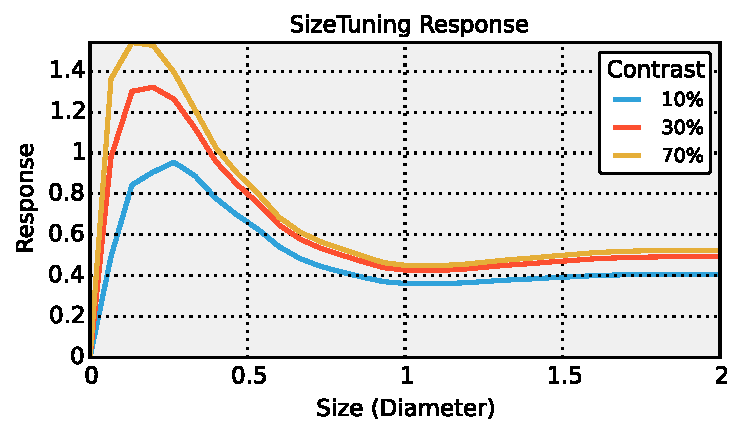
\includegraphics[width=0.5\textwidth]{./results/SCAL/LGN_SizeTuning.pdf}
	\caption[SCAL model size tuning curves]{LGN neuron size tuning
      representing the response of a stereotyped LGN neuron to a
      sinusoidal grating disk stimulus with increasing contrast. The
      tuning curves demonstrate a small but noticeable shift toward
      larger size preferences at lower contrasts.}
	\label{LGNSizeTuning}
\end{figure}

\begin{figure}
	\centering
        \includegraphics[width=1.0\textwidth]{./results/SCAL/LGN_DoG.pdf}
	    \caption[SCAL model size tuning DoG
          fit.]{Difference-of-Gaussian model goodness of fit
          comparison for SCAL size tuning curves. A) LGN
          area-summation curve (gray) fitted using a subtractive
          (blue) and divisive (red) integrated DoG model. B) Fraction
          of explained variance ($r^2$) of the subtractive and
          divisive DoG models.}
	\label{LGNSizeFit}
\end{figure}

Since LGN responses in this model do not have any source of
variability we cannot compare the distributions directly. To compare
the responses with the experimental results we will treat the 10\%
contrast response as the low contrast response and 70\% contrast as
the high contrast response. This matches the experiment where the
contrast with 20-50\% and 70-90\% of the maximal contrast are taken as
low- and high-contrast responses respectively. To compare the data
directly to the experimental data, we have overlaid the low and high
contrast estimates of the excitatory and inhibitory constant directly
on experimental data from \cite{Sceniak2006} (see
\ref{LGNDistribution}).

The excitatory space constant $a$ was estimated at $0.16\degree$ at
high contrast, expanding to $0.294\degree$ at low contrast. The
inhibitory or surround space constant on the other hand was
$0.62\degree$ at high contrast and $0.56\degree$ at high contrast. 
These values fall well in the distributions that have been measured in
experiments, even if they are reaching toward the smaller end of what
was measured in thalamocortical afferents in the visual cortex.

\begin{figure}
	\centering   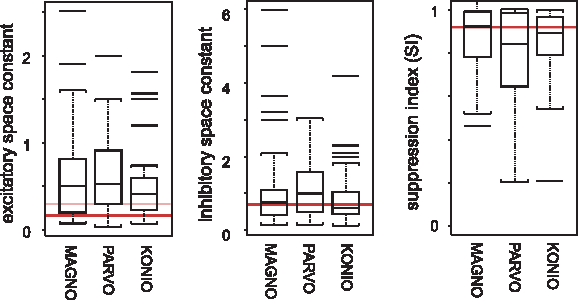
\includegraphics[width=1.0\textwidth]{./Sceniak_LGN_Distribution.pdf}
	\caption[Distribution of excitatory and inhibitory in
      thalamocortical afferents.]{Distribution of excitatory and
      inhibitory space constants in thalamocortical afferents
      reproduced from \cite{Sceniak2006} (in macaque) and overlaid
      with estimates obtained from the SCAL LGN model at low contrast
      (pink) and high contrast (dark red).}
	\label{LGNDistribution}
\end{figure}

\subsubsection{Frequency Tuning}

The frequency tuning of LGN neurons in macaque V1 is strongly
correlated with the size tuning, nonetheless we want to confirm the
frequency tuning curve matches what is seen in experiment. Therefore
we replicate the frequency tuning measurements performed by
\cite{Levitt2001}. The sinusoidal gratings used for measurement were
presented in a $2x2^{\circ}$ area, well beyond the size of the
surround field. The resulting frequency tuning curves are shown in
\ref{LGNFrequencyTuning}, showing a slight contrast dependent shift
toward higher frequencies at higher contrasts.

\begin{figure}
	\centering
    \includegraphics[width=0.5\textwidth]{./results/SCAL/LGN_FrequencyTuning.pdf}
	\caption{LGN neuron frequency tuning representing the response of
      a stereotyped LGN neuron to a $2x2^{\circ}$ sinusoidal grating
      stimulus at a wide range of contrasts.}
	\label{LGNFrequencyTuning}
\end{figure}

We compare the spatial frequency preference of the model LGN directly
with a scatter plot of spatial frequency preferences against
eccentricities, again demonstrating that we are well within the
empirically validated distribution of values (see
\ref{LGNFrequencyLevitt}).

\begin{figure}
	\centering
    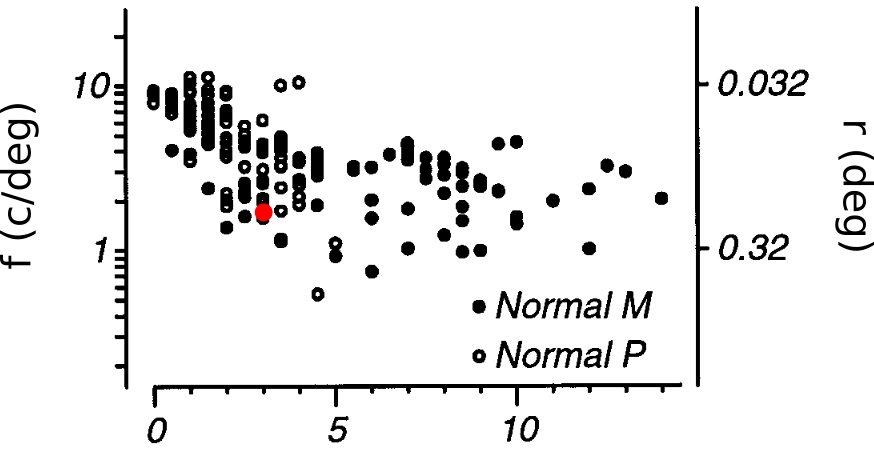
\includegraphics[width=0.8\textwidth]{./LGN_FrequencyLevitt.png}
	\caption[Spatial frequency preference in SCAL compared to
      experiment. Adapted from \cite{Levitt2001}.]{Plot of preferred
      frequency tuning of neurons in the LGN of normally reared and
      visually deprived macaque monkeys overlaid with the optimal
      spatial frequency of the stereotyped SCAL LGN neuron (red
      circle). Adapted from \cite{Levitt2001}.}
	\label{LGNFrequencyLevitt}
\end{figure}

\subsection{The V1 model}

Before going into the spatial calibration of the V1 stage of SCAL
model, we will first review how the model self-organizes into a
smooth, high-quality orientation map. The model was in most cases
simulated as a $4^\circ x 4^\circ$ area, which corresponds to around
$12 mm^2$ of cortical area. After training using one of the three
datasets a wide range of measurements were performed to confirm the
model developed correctly and exhibited the same properties as GCAL.

The orientation map, receptive fields and orientation tuning curve for
the fully developed model are shown in \ref{SCALORTuning}. These
results demonstrate that the final spatially calibrated model still
exhibit good quality orientation maps, contrast independent
orientation tuning and very clear oriented lobes in individual
receptive fields. Comparing the robustness of map organization to the
GCAL model will be performed later on, when we are looking at the
properties that make a model robust to a wide range of inputs.

% jbednar: B would be better in red/blue, as would fig 4.13, 5.4, etc.
\begin{figure}
	\centering
    \includegraphics[width=1.0\textwidth]{./results/SCAL/SCAL_V1_ORTuning.pdf}
	\caption[Orientation tuning properties of the SCAL model.]{SCAL
      model orientation tuning properties after presenting 20,000
      oriented Gaussian patterns. A) Orientation map measured by
      presenting sine gratings at the optimal spatial frequency to the
      model, along with the locations of the receptive fields shown in
      B. B) Gabor fits to receptive fields measured using sparse
      random noise. C) Orientation tuning curve of a single neuron
      across contrasts, demonstrating largely contrast dependent
      orientation tuning.}
	\label{SCALORTuning}
\end{figure}

\subsection{V1 Spatial Calibration}

A neuron in primary visual cortex receives input from a variety of
sources, including feedforward connections from the LGN, horizontal
connections from within V1 and feedback connections from extrastriate
cortex as seen in Figure \ref{RFstruct}. Translating the fully
complexity of the known spatial profiles of these different synaptic
inputs to the visual cortex therefore requires integrating a wide
range of information from different sources including anatomical,
electrophysiological and optical imaging. Not only will this let us
build a model that corresponds more closely to the macaque visual
cortex in vivo, but also let's us cross-validate the experimental
data, highlighting potential discrepancies.

The first step to bridge measurements from different sources will be
to establish a well defined mapping from visual space to cortical
space. From there we will evaluate the different sources of
measurement, replicating the measurements in the model and comparing
the results. Finally we will summarize the model parameters that were
chosen and will be carried over to later models.

\subsubsection{Magnification factors \& Hypercolumn Distance} \label{SCALHypercolumns}

As we outlined above most studies of V1 particularly in the surround
modulation literature focus on parafoveal regions between $2-5\degree$
in eccentricity. Therefore we have chosen to model the region around
$3\degree$ in eccentricity. This already gives us a number of
constraints, first of all giving us an approximate V1 magnification
factor of 3 mm/\degree as described by \cite{VanEssen1984} and shown in
Table \ref{MFs}. This means that each degree of visual space
corresponds to 3 mm on the cortical surface at this particular
eccentricity. However without an independent measure of the cortical
space this conversion factor is still entirely arbitrary. Therefore we
make use of the fact that the hypercolumn distance between orientation
columns in V1 is well defined by numerous studies.

% jbednar: would be more readable if the citations would fit into the
% first column; seems like they might
\begin{table}
\centering
\begin{tabular}{l | c c}
  \hline
  \hline
  Visual Area     & Magnification Factor ($mm/\degree$) & Anisotropy Index \\
  \hline
  Retina$^1$      & 0.223                            & -                      \\
  LGN$^2$         & 0.324                             & 1.0-2.0                \\
  V1$^3$          & 2.54-3.545                       & 1.0-3.0                \\
  \hline
\end{tabular}
\caption[]%
{Magnification Factors and Anisotropy Index associated with different
  visual areas at $3\degree$ eccentricity estimated from areal and
  linear magnification factor equations. Footnotes: $^1$ -
  \cite{Perry1985}, $^2$ - \cite{Connolly1984}, $^3$ -
  \cite{VanEssen1984}}
\label{MFs}
\end{table}

To give actual scale to our model, we can therefore measure the
orientation map hypercolumn distance. Using estimates provided by the
Wolf group the hypercolumn distance in macaque V1 has been estimated
at roughly ($710 \pm 50 \mu m$). By combining this information with
the magnification factor we can establish that we'd expect roughly 4.2
hypercolumns per visual degree ($3 mm/\degree * 710 \mu m$). We will also
define an acceptable range of hypercolumn cycles per degree to ensure
later models do not diverge too far from the spatial tuning
implemented here. Taking the confidence intervals for both the
magnification factor and hypercolumn distance into account the
acceptable range of hypercolumns per sheet coordinate is between 3.29
and 5.3.

The hypercolumn distance in the model was calculated by taking the 2D
Fourier transform of the orientation map, reducing it to one dimension
and applying a least-squares fit of a Gaussian curve with additional
linear and quadratic terms (see \cite{Kaschube2010} for more
details). A sample fit to an SCAL orientation map can be seen in
Figure \ref{SCALhypercolumns}. The final model has ~4.03 hypercolumns
per visual degree, which falls well within the acceptable range.

Based on that measurement we can now explicitly state that 1 visual
degree corresponds to 3 mm in the model, which will let us
independently confirm that the extent of the final model weights are
consistent with experimental measurements but also internally
consistent with the size tuning response of the model. The next steps
will be to evaluate feedforward and lateral connections independently.

\begin{figure}
	\centering
        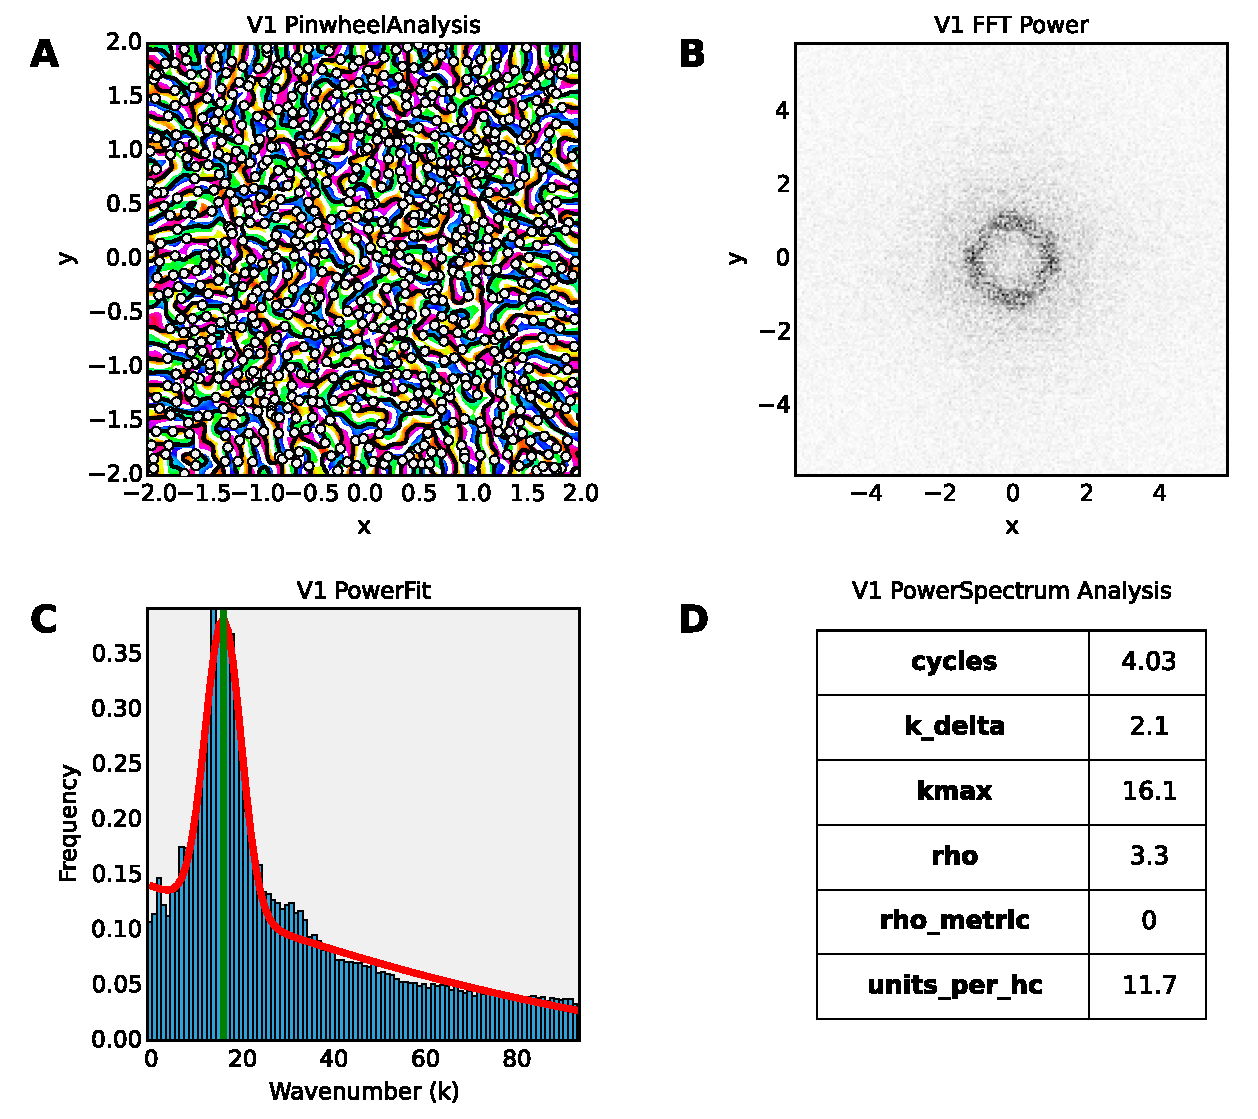
\includegraphics[width=1.0\textwidth]{SCAL_hypercolumns.pdf}
	\caption[Hypercolumn and pinwheel density fitting procedure and
      results.]{Hypercolumn and pinwheel density fitting procedure. A)
      Orientation map in V1 overlaid with real and imaginary contours
      and pinwheels at their intersections. B) 2D FFT of the
      orientation map showing a ring identifying the periodicity of
      the map. C) 1D histogram of the FFT along with Gaussian fit
      marking the best fit hypercolumn distance. D) Summary table
      showing various parameters of the fit, along with pinwheel
      density ($\rho$) which classifies the quality of the map.}
	\label{SCALhypercolumns}
\end{figure}

\subsubsection{Feedforward}

The afferent input from the lateral geniculate nucleus is the main
driver of responses in the primary visual cortex. It is therefore
crucial in determining the size tuning profile of the visual cortex.
The \ref{AfferentBackground} discussed how the integrative area of a
neuron in V1 is made up of the combined integrative area of
thalamocortical projections and retinogeniculate projections.

\paragraph{Area summation}

The first step in the fitting procedure was to repeat the protocols
applied to the LGN, i.e. measuring area summation curves and fitting
DoG models to the results. Using this approach we obtained a large
number of size estimates for the excitatory and inhibitory kernels
contributing to the V1 response, which we can compare to the results
obtained from comparable studies in macaque visual cortex.

\begin{table}
  \centering
  \begin{adjustbox}{width=1\textwidth}
  \begin{tabular}{l | l l l l}
    Measurement              & Literature            & Species & Layer & Diameter \\
    \hline
    V1 hsRF                  & \cite{Levitt2002}     & macaque & 2-6 & $1.0 \pm 0.1\degree$ (0.15 - 1.1) \\
    \hline
    V1 Excitatory DoG fit    & \cite{Levitt2002}     & macaque & 2-6 & $0.9\degree$ \\
                             & \cite{Sceniak2001}    & macaque & 2-6 & $2.0\degree$ \\
                             & \cite{Cavanaugh2002}  & macaque & 2-6 & $1.4\degree$ \\
                             & \cite{Solomon2002}    & macaque & not stated & $0.94\degree$ \\
    \hline
    V1 Inhibitory DoG fit    & \cite{Levitt2002}     & macaque & 2-6 & $1.9\degree$ \\
                             & \cite{Sceniak2001}    & macaque & 2-6 & $4.4\degree$ \\
                             & \cite{Cavanaugh2002}  & macaque & 2-6 & $2.7\degree$ \\
                             & \cite{Solomon2002}    & macaque & not stated & $2.97\degree$ \\
    \hline
  \end{tabular}
  \end{adjustbox}
  \caption{Functional estimates of V1 receptive field size using
    Difference-of-Gaussian models.}
  \label{electrophystable}
\end{table}

The table \ref{electrophystable} summarizes the mean results obtained
by these studies, with a general agreement of an afferent integration
field that spans about $1\degree$ in diameter, with inhibitory
surround that is on average about two times larger at about 
$2\degree$. The most thorough analysis being performed by
\cite{Cavanaugh2002}, who fitted a number of variants of the model. In
addition to measuring integrative area of V1 neurons in visual space
they converted the results into cortical space using the known
magnification factor. In \ref{CavanaughDistribution} the results from
the model, also converted to cortical space are compared to these
distributions, showing less diversity but general agreement on mean
and median values.

\begin{figure}
	\centering
        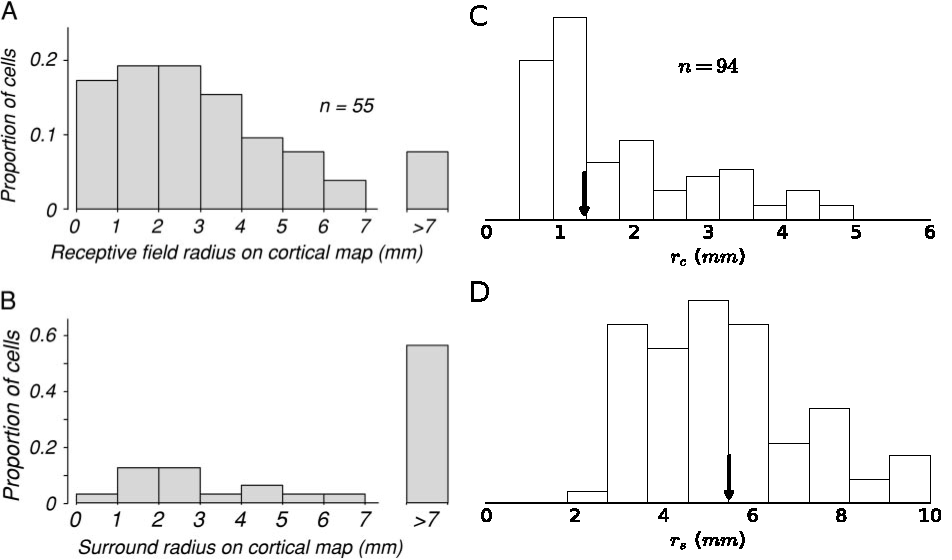
\includegraphics[width=1.0\textwidth]{Cavanaugh_V1_Distributions.pdf}
	\caption[Distribution of V1 Difference-of-Gaussian space constants
      measured by \cite{Cavanaugh2002} compared to SCAL
      model.]{Comparison between the distributions of space constants
      estimated by \cite{Cavanaugh2002}, converted from visual angle
      to cortical space and the equivalent measurements applied to the
      model. A, C) Distributions of maximal integration area radii.
      B, D) Distributions of suppressive surround area radii. }
	\label{CavanaughDistribution}
\end{figure}

Additionally we also compare the shift in size tuning preference
between low and high contrast conditions, between experiment
\citep{Sceniak1999} and the model. In addition to the SCAL model, the
analysis also includes results from GCAL, which employs subtractive
rather than divisive inhibition. The results highlight that the GCAL
model does not really exhibit any meaningful size tuning shift between
low and high contrast. Additionally both model scatter plots clearly
highlight the lack of diversity in the model. Generally however, the
results are qualitatively very similar between SCAL and the
experimental data, showing a mean shift and distribution of shifts
that is very similar (2.2x shift in experiment vs. 1.8x in the model).

\begin{figure}
	\centering
        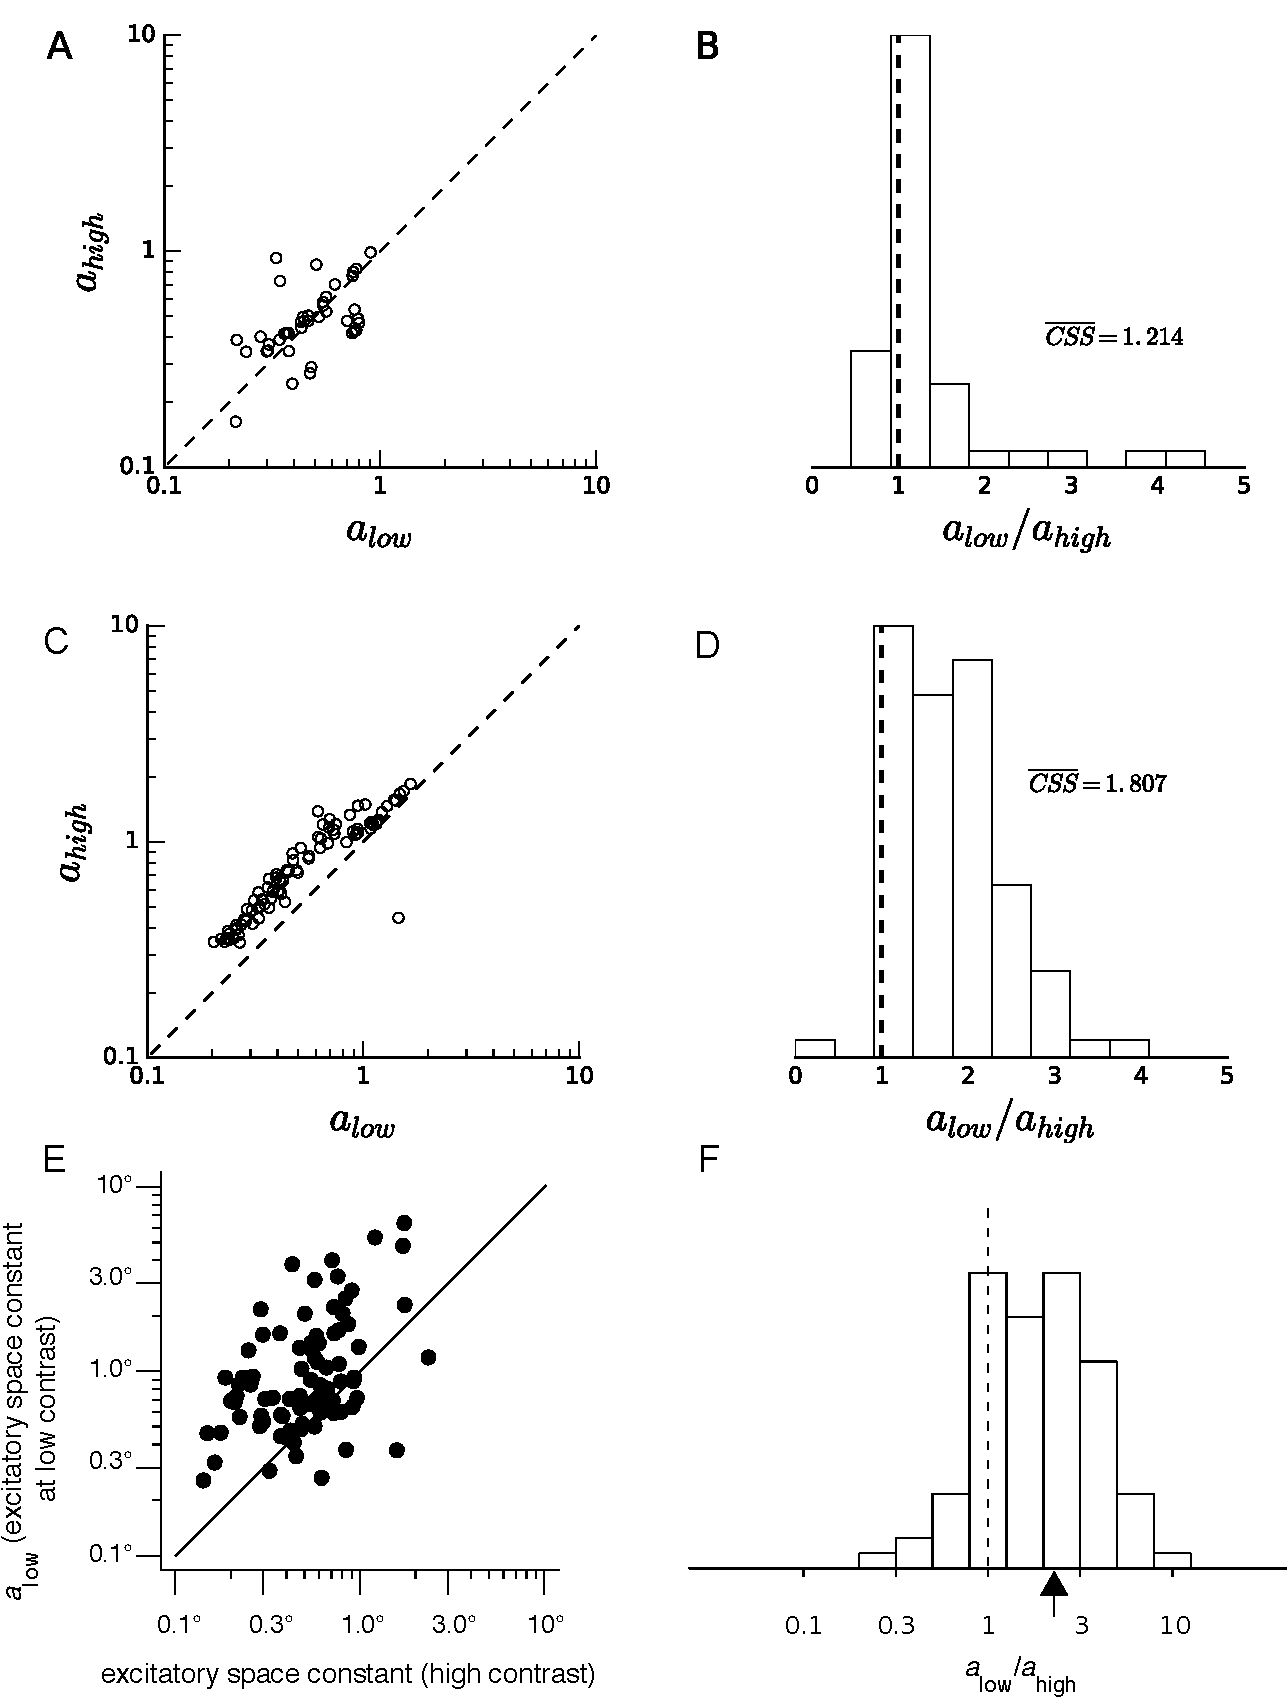
\includegraphics[width=0.8\textwidth]{./V1_DoG_Contrast.pdf}
	\caption[Contrast dependent size tuning shifts compared between
      GCAL, SCAL and experimental results from
      \cite{Sceniak1999}.]{Comparison between contrast dependent size
      tuning shifts between the GCAL model (A, B), the SCAL model (C,
      D) and experimental results from \cite{Sceniak1999} (E, F). A,
      C, E) Scatter plot of DoG excitatory constant at low and high
      contrast in experiment and the model respectively. B, D, F)
      Distribution of contrast dependent shift in excitatory
      constant.}
	\label{ContrastShift}
\end{figure}

Finally we investigate the distribution of suppression indices, which
shows a similar mean value but also highlights the complete lack of
unsuppressed cells.

\begin{figure}
	\centering
        \includegraphics[width=0.6\textwidth]{./results/SCAL/SCAL_V1_SI.pdf}
	\caption{Distribution of Suppression Index (SI) values under
      high-contrast stimulus condition.}
	\label{SCALSI}
\end{figure}


\paragraph{Receptive Fields}

In addition to measuring the area summation responses of V1 neurons we
can also assess the spatial profile of V1 receptive fields by mapping
them using reverse correlation techniques. After mapping the receptive
fields using 5000 sparse, random stimuli the results were fit using
the simple Gabor model described in \ref{rffitting}. In addition to
once again confirming the spatial frequency preference of the neurons,
we compared the $n_x$ and $n_y$ ratios of the neurons to equivalent
measurements in macaque \citep{Ringach2002b} and cat
\citep{Jones1987}.

The results show a similar general shape but also demonstrate a shift
toward greater $n_x$ values as compared to the experimental data.

\begin{figure}
	\centering
        \includegraphics[width=1.0\textwidth]{./results/SCAL/RF_nxny.pdf}
	\caption[Relative elongation and width of V1 receptive fields. A
      comparison between SCAL, cat V1 \cite{Jones1987} and macaque V1
      \cite{Ringach2002b}.]{Scatter plot of receptive field $n_x$ and
      $n_y$ values, representing the width and length of the receptive
      field relative to the period of the grating underlying the Gabor
      fit respectively. Comparison between results from
      \cite{Ringach2002b} in macaque V1 (circles), \cite{Jones1987} in
      cat V1 (crosses) and in the SCAL model (squares).}
	\label{RFFits}
\end{figure}

\subsubsection{Intracortical connectivity}

We have already settled that afferent activity is the major driver of
responses in primary visual cortex but intracortical, recurrent
connections between neurons are though to provide significant
modulatory influences on V1 responses. Precisely breaking down the
contributions of specific connections, particularly when taking into
account the cell types is much more difficult, particularly because
experimental data is much more scarce. In \ref{InhibitoryBackground}
we summarized the potential role of different inhibitory subclasses,
however beyond some estimates of the maximum extent of the axonal
projections from different cell classes \citep{Kisvarday1993,
  Kisvarday1997a, Budd2001, Buzas2001}, very little is known about
their spatial profile. The extent of excitatory projections between V1
neurons are better studied, with a range of estimates for the maximum
extents \citep{Angelucci2002} and even some models of the spatial
profile of connections \citep{Buzas2006} being available.

We summarize various anatomical estimates of the extents and spatial
distribution of intracortical connections in
\ref{anatomicaltable}. Note that due to the lack of data a lot of
these estimates were obtained in cat V1, which means we have to
extrapolate these results to macaque V1.

\begin{table}
  \centering
  \begin{adjustbox}{width=1\textwidth}
  \begin{tabular}{l | l l l l}
    Connection               & Literature            & Species & Layer & Diameter \\
    \hline
    LGN-V1 Afferents         & \cite{Angelucci2002c} & macaque & 4C$\alpha$ & $0.8-1.6\degree$ \\
                             & \cite{Angelucci2006a} & macaque & 4A/4C$\beta$ & $0.91 \pm 0.041\degree$ \\
    \hline
    V1 local excitation      & \cite{Buzas2006}      & cat      & 2-4 single cell & $288 \mu m$ \\
                             & \cite{Buzas2006}      & cat      & 2-4 population  & $520 \mu m$ \\
    \hline
    V1 basket cells          & \cite{Buzas2001}      & cat      & 2-6 & $0.7-1.9\degree$ \\
                             & \cite{Buzas2001}      & cat      & 2-6 & $0.76-2.6 mm$ \\
    \hline
    V1 long-range excitation & \cite{Angelucci2002}  & macaque  & 2/3 & $6\pm 0.7 mm$ (3-9) \\
                             &                       &          & 4B/4C$\alpha$ & $6.7 \pm 0.7 mm$ (4.7-10) \\
                             &                       &          & population & $2.47 \pm 0.3\degree$ \\
                             & \cite{Buzas2006}      & cat      & 2/3 & $6 mm$ \\
    \hline
  \end{tabular}
  \end{adjustbox}
  \caption{Anatomical estimates of the spatial profiles of V1
    connectivity from macaque and cat.}
  \label{anatomicaltable}
\end{table}


\paragraph{Excitatory Connections}

The literature has had a much harder time of picking apart the
contribution of intracortical and particularly the patchy lateral
connectivity found in V1 so to confirm that these connections have
developed as expected is to compare it to anatomical measurements.
For this purpose we will be fitting a descriptive model, developed by
\cite{Buzas2006} to the lateral connectivity data.

The distance of long-range connectivity varies considerably across
species so using some anatomical estimates from macaque we will
attempt to refine our estimates of the long-range oriented
component. Anatomic data suggests that the spatial spread of lateral
connections can be anywhere between 3-10 mm (on average 6-7 mm) in
total length \citep{Angelucci2002}. Along its principal axis the
visuotopic mono-synaptic spread of V1 horizontal connections has a
mean of \(2.47^\circ\) \(\pm\) \(0.3^\circ\). This falls well within
the range of estimates for the lsRF as published in a number of
studies \citep{Sceniak1999, Sceniak2001, Shushruth2009}, which employed
the iDoG protocol.

\begin{figure}
	\centering
        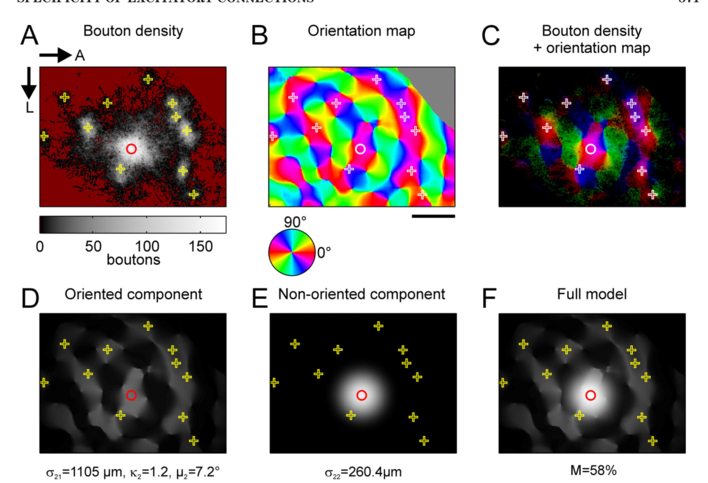
\includegraphics[width=1.0\textwidth]{Buzas.png}
	\caption{Lateral excitatory projection bouton density and
          orientation maps in layer 2/3 of cat V1 fit using a Gaussian
          and von Mises model, replicated from \cite{Buzas2006}.}
	\label{Buzas}
\end{figure}

The model that was used to fit the lateral weights describes the
patchy lateral connectivity found in layer 2/3 of V1 as a function of
two distinct components. A short range isotropic Gaussian pattern and
a long range pattern, defined as a von Mises function, which is
combined with the orientation map. The model therefore assumes that
lateral connectivity develops as a function of both the proximity in
space but also along a particular feature dimension, in this case the
orientation. The equations underlying this model and an extension,
which also exposes the aspect ratio of the long-range Gaussian kernel
are described in \ref{BuzasEquations}.

The full model fitting procedure for an experimentally traced lateral
connection field is shown in Figure \ref{Buzas}. By applying this
fitting procedure we can effectively estimate the spatial extents of
both the local isotropic local kernel and the long-range excitatory
kernel. The figure \ref{LatFits} demonstrates what one such fit looks
like for the SCAL model, while the full distribution of local and
long-range kernel values is shown in \ref{LatDist}. Note that the
weight array that is being fit has been thresholded at the 70th
percentile of non-zero values to ensure the weight matrix more closely
resembles the bouton density maps obtained by \cite{Buzas2006}.

\begin{figure}
	\centering
        \includegraphics[width=1.0\textwidth]{./results/SCAL/SCAL_vonMises_Fits.pdf}
	\caption[Combined Gaussian+vonMises model fits to lateral
      connectivity of the SCAL model.]{Example fits obtained by
      fitting Gaussian and von Mises distributions to the thresholded
      long-range lateral weights. A) The thresholded long-range
      lateral weight matrix (at the 70th percentile). B, C) Example
      fits using the von Mises orientation model with and without an
      aspect parameter. D, E) Error between the fits and the
      thresholded weight matrix pattern.}
	\label{LatFits}
\end{figure}

The results of our fitting procedure shown in Figure \ref{LatDist}
show good correspondence with these experimental estimates with a mean
long-range connectivity that has a spatial constant of around $1645 \mu m$
but extends beyond that with our cut-off defined at
$2.5\degree$ or $7.5 mm$. The model without aspect fits the
experimentally obtained long-range spatial constant more closely but
neither extends to the furthest reaches of the lateral connection
field. The local excitatory kernel provides a reasonable fit to
experimental estimates with a mean local excitatory kernel with a
spatial constant of around $221 \mu m$, compared to the $280 \mu m$
estimated in cat V1 \citep{Buzas2006}. However most neurons exhibit
much smaller local kernels and the distribution seems to be
distributed bi-modally.

\begin{figure}
	\centering
        \includegraphics[width=1.0\textwidth]{./results/SCAL/SCAL_Buzas_Distributions.pdf}
	\caption[Distribution of spatial constants obtained by fitting
      Gaussian+vonMises model.]{Distribution of spatial constant
      obtained by fitting the \cite{Buzas2006} von Mises+Gaussian
      model to long-range lateral excitatory connections developed as
      part of the SCAL model.}
	\label{LatDist}
\end{figure}

Finally we can evaluate in how far the orientation preference and
selectivity of the post-synaptic neuron predicts the long-range
lateral connections it receives. Specifically we can evaluate how
closely the $\kappa$ value of the von Mises fit, which represents the
bandwidth of the kernel in the orientation domain, is correlated with
the orientation selectivity of the neuron. The relationship between
these two variables is shown in \ref{LatORKappa}, and clearly predicts
that the orientation specificity of the lateral connections received
by a V1 neuron is highly dependent on the orientation selectivity of
the neuron (spearman $\rho=0.59$, $p<1e-184$).

\begin{figure}
	\centering
        \includegraphics[width=1.0\textwidth]{./results/SCAL/SCAL_vonMises_ORSel.pdf}
	\caption[Relationship between the width of vonMises distribution
      in the lateral connectivity model and the orientation
      selectivity of the neuron.]{Scatter plot of the $\kappa$
      variable of the von Mises distribution and the orientation
      selectivity of each neuron, showing a clear relationship between
      the orientation specificity of patchy lateral connections and
      the post-synaptic neurons orientation selectivity. The points
      are additionally colored by their goodness of fit and marginal
      histograms of the distributions of the $\kappa$ and orientation
      selectivity are provided. Fits with an $R^2$ value below 0.3
      were rejected.}
	\label{LatORKappa}
\end{figure}

\subsubsection{Inhibitory connectivity}

Since the SCAL model does not have distinct populations of V1 we will
consider the joint spatial and orientation distribution of basket
cells in order to determine the inhibitory profile and compare model
to experiment. \cite{Kisvarday1997a} provide the best known estimates
for the spatial distribution of inhibitory basket cells, having
injected tracers much more conservatively than previous studies. Their
estimates indicate that inhibitory projection in cat V1 extend no
further than 1.5-2 mm with most synaptic boutons being distributed in
a central regions approximately 1 mm in diameter. In the absence of
any precise fits, equivalent to the Gaussian and von Mises model
available for the excitatory connectivity, we restrict inhibitory
connectivity to a conservative 1.2 mm in diameter.

By binning the strength of connections by their distance and the
orientation difference between pre- and post-synaptic neurons we can
at least qualitatively assess how closely the model distribution
matches experimental bouton density maps. The analysis breaks down the
spatial distribution of connections targeting iso-, oblique and
cross-orientation regions, comparing against the equivalent analysis
performed by \cite{Kisvarday1997a} in cat area 17. While we are
restricting the inhibitory connectivity to a smaller region the
experimental results highlight again that most weights fall into the
central region. Additionally we can see that the distributions of
weights broken down by distance are qualitatively very similar, with
most of the weight in the iso-orientation case being centered near the
center, while oblique and cross-orientations are strongest at medium
ranges.

\begin{figure}
	\centering
        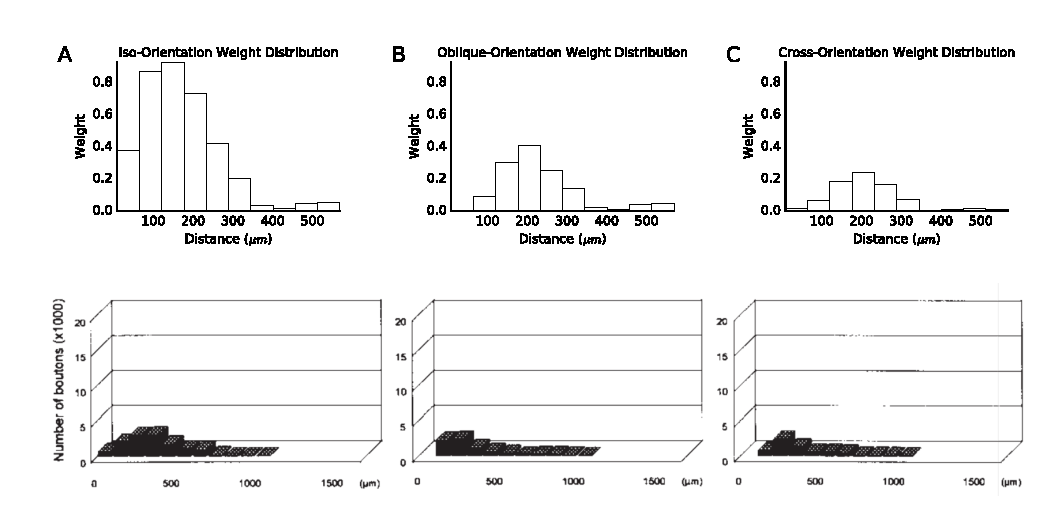
\includegraphics[width=1.0\textwidth]{./SCAL_Inh_Distribution.pdf}
	\caption[Spatial and orientation distribution of the lateral
      inhibitory weights in SCAL.]{Distributions of inhibitory
      projections as a function of space broken down into
      iso-orientation, oblique orientation, and cross orientations
      relative to the orientation preference of the post-synaptic
      neuron.}
	\label{LatDist}
\end{figure}

\subsubsection{Sparsity of connections}

The implementation of the GCAL and SCAL models has generally meant
that neurons densely innervate neurons within the defined spatial
extent. However from experimental studies it is known that neurons
actually only make fairly sparse contact to neurons around them and
once the initial sprouting and pruning phase of development is over it
is generally much harder to form new connections. In particular we
know that a V1 neuron is only contacted by a fairly small number of
afferent projections from the LGN and that lateral projections while
very dense innervate only a small fraction of neurons around
them. This has profound implication for development because neurons
have much sparser input than is assumed in these models, secondly it
can strongly affect the development of the model because once
connections have been formed it is much more difficult to shift the
synaptic weights to some other location.

A detailed investigation into the processes underlying sprouting and
pruning and the competition for afferent inputs would be a thesis in
itself. However for computational purposes but also to test the
robustness of the model we implemented a simple form of sprouting and
pruning, which starts out with a densely connected network and slowly
prunes away connections while also generating a small number of new
weights.

In this way we can demonstrate that sparsity of connections can indeed
increase the robustness of the model and that how true long-range
patchy connectivity akin to the thresholded version used in the von
Mises model fitting procedure can emerge from the model.

\section{Discussion}

In this chapter we set out to spatially calibrate the GCAL
developmental model in order to cross-validate known measurements of
the spatial profile of afferent, excitatory and inhibitory connections
in the primary visual cortex. Additionally we wanted to explore how
the intra-areal connectivity in the cortex can give rise to a Mexican
hat like profile, which is thought to underlie the organization of the
cortical neurons into smooth topographic maps, which optimally map
features in the sensory input onto the surface of the cortex.

In the literature review we had established that long-range
connections in the cortex are almost exclusively excitatory. However
the spatial scales involved in mediating Mexican hat like connectivity
are well below the long-range excitatory connections, which can often
span many hypercolumns. By incorporating the empirically determined
spatial scales of the model we were able to establish that the
relatively long projections originating from the basket cell
population in V1 is sufficient to account for the Mexican hat
profile. At the same time we show that long-range surround suppression
cannot be effected directly by these projections and must instead by
mediated by a di-synaptic mechanism, via the long-range excitatory
projections.

First we will review how we determined the spatial parameters of the
SCAL model, before critically reviewing the experimental measurements
given in the light of the model results. This will let us highlight
issues with DoG fitting procedures employed to fit area summation
curves in visual cortex and call into questions some conclusions made
about the source of contrast dependent size tuning shifts. Finally we
will discuss the model of lateral excitatory connectivity and how the
addition of an aspect parameter can help us quantify the isotropy of
patchy lateral connectivity in a way that can easily be applied to
experiments.

\subsection{The LGN Model}

In spatially calibrating the early stages of the model, roughly
corresponding to the retinal ganglion cell and lateral geniculate
nucleus, we relied mostly on electrophysiological estimates of the
size and area summation curves of the neurons. In doing so we had two
primary aims, first of all since we chose only a single spatial filter
rather than a distribution for computational reasons. Later models can
easily add further diversity to the model by drawing the the spatial
constants of the center-surround filters from a distribution. In the
absence of this diversity we chose a spatial filter size that had to
have several important properties.

The first was that the chosen values should not diverge too far from
the values obtained by fitting a DoG model to area summation
curves. We confirmed this was the case and plotted the results
compared to the empirical data obtained from \cite{Sceniak2006},
finding the values at the lower end of the distribution.

The second constraint was that the spatial frequency preference of the
neurons could not be too low in order to allow V1 neurons to integrate
over at least one cycle of the main spatial frequency preference. This
meant that the preferred spatial frequency of the network should fall
somewhere between 1 and 2 cycles per degree of visual angle. Again we
confirmed this was the case and compared the result to similar results
obtained by \cite{Levitt2001} in the visual cortex of macaques.

The extent of the gain control projection in LGN could not be
experimentally verified as there is little to no data about the
precise anatomical profile of inhibitory neurons in the LGN. Therefore
we chose a value that would allow normalize everything within the
receptive field of a single V1 neuron.

The final model parameters are summarized in \ref{LGNTuning} and
visualized in Figure \ref{LGNDiagram}. In future this model may be
extended by drawing the extent of these afferent connections from a
distribution. For the purposes of this thesis, this level of
calibration is sufficient however and will provide the V1 model with
input that is roughly at the desired spatial scale.

\subsection{The V1 Model}

The V1 model that was introduced in this chapter is able to replicate
a wide range of experimental results and provides a much closer match
to experimental results than the existing GCAL model. In addition to
spatially calibrating the extents of afferent and lateral connections,
the model is also the first developmental model that uses divisive
rather than subtractive inhibition. The divisive model provides a much
better account of size tuning responses, which shift to larger
integrative areas depending on the contrast, which agrees with a wide
range of existing models. We also showed that the extents of
inhibitory basket cells is sufficient to account for the Mexican hat
profile that has long been used to explain the organization of neurons
into topographic feature maps by pulling together activity locally and
suppressing it in nearby regions, which leads to a smooth mapping of
different feature preferences across the cortical surface.

However, in exploring this model we have also encountered clear
limitations. The most important of which is the lack of distinct
excitatory and inhibitory populations. Apart from directly violating
Dale's law, this poses a serious problem for a developmental model.
This is because Hebbian learning will ensure the strength and spatial
profile of the neural connections is dependent on the response
properties of the neuron and different cell types may respond very
differently. This has made it difficult to directly compare the
lateral connectivity in the model.

\subsubsection{Differences to GCAL}

There are a number of major changes between the GCAL model and the
SCAL model that was introduced in this chapter. As we have already
emphasized the SCAL model operates on divisive rather than subtractive
inhibition. While inhibition in the brain generally has both divisive
and subtractive effects, the divisive normalization paradigm has shown
tremendous success in explaining a wide range of effects including
modulatory effects, contrast dependent changes in responses,
decorrelating the inputs and even effects associated with visual
attention \citep{Cavanaugh2002a, Graham2011, Carandini2012,
  Reynaud2012, Coen2015}.

The other aim was to move away from other unrealistic
mechanisms. While the model does not learn continuously it no longer
artificially resets the activity between stimulus presentations or
saccades. The model now behaves more continuously with no hard reset
between stimulus presentations. Instead the model activity from a
previous step decays at the start of a new presentation and is usually
extinguished completely by the time it reaches V1.

While all the spatial profiles have changed in some way or another the
most significant change was the size of the afferent field relative to
the lateral connections in V1. While the receptive fields of neurons
in GCAL generally only subtended only a single hypercolumn, the
receptive fields in SCAL span somewhere between 3-4
hypercolumns. Long-range connectivity in the GCAL model therefore
generally connected neurons with non-overlapping receptive fields,
while the SCAL model highlights that this is generally not the case in
parafoveal regions of macaque V1. A good portion of the lateral
connectivity field actually connects neurons with significantly
overlapping connection fields and only a portion of long-range patchy
connections reaches outside the neurons receptive field. This has
significant implications for the function of these connections, rather
than purely reflecting the co-occurence of stimuli the patchy
connections will strongly mirror the response of the neuron
itself. This suggests that lateral connections are involved in
improving the encoding of the local stimulus in addition to mediating
true surround influences.

Despite some of these limitations the model exhibits very robust
development under varying stimulus conditions and still exhibits all
the nice properties of the GCAL model, including contrast invariant
orientation tuning as well as robust, yet adaptive self-organization.

\subsubsection{Size tuning}

A major component of the analysis we applied here was in comparing
applying a Difference-of-Gaussian model to the area summation curves
and comparing the results to equivalent experimental data. Since the
model itself does not exert any long-range influences any changes in
the fit is must likely mediated by the relatively short-range
connections in the model. However we did find significant shifts in
the integration area depending on the contrast level in the SCAL model
but not in the GCAL model. This suggests suggest the contrast
dependent shifts in effective integration area can be explained by
changes in the relative gain of the center and surround component in a
ratio-of-Gaussians model, just as was proposed by
\cite{Cavanaugh2002}. It is therefore not necessary to invoke
integration over a larger area via long-range lateral connections as
was suggested by the experimental work by \cite{Levitt2002} and
\cite{Sceniak2001} and translated into a model by
\cite{Schwabe2006}. This does not mean however that long-range lateral
connections do not have any influence. Indeed it is difficult to
envision how the model can mediate any longer range feature specific
excitation and inhibition without corresponding long-range projections
between neurons, which are themselves tuned for those specific
features.

\subsubsection{Lateral Connectivity}

\paragraph{Excitatory}

In addition to fitting the response properties of the V1 neurons this
chapter also demonstrated how the anatomical distribution of synaptic
boutons can be compared to the lateral connectivity in the model. By
fitting a model made up of a local Gaussian kernel and an orientation
dependent long-range kernel, first devised by \cite{Buzas2006}, to the
data we are able to achieve good fits demonstrating that the lateral
connectivity captures the statistics of the visual input. In addition
the results indicated that at least the extent of the long-range
connectivity is consistent with experimental results. However, the
short-range kernels were significantly smaller in scale than what we
would expect from experiment. There are multiple factors that could
account for this difference. The main issue being that the model only
captures one population of cells, which generally display a high level
of feature selectivity. More diversity, such as the introduction of
unselective inhibitory cells could explain larger and more weakly
tuned local connections. Another factor that could play a role is that
neurons in macaque V1 are generally much more dense and the
hypercolumn distance considerably shorter. With relatively larger
hypercolumns we could also expect that the excitatory connectivity
grows in size. Finally, the development of connectivity in the model
is driven entirely by Hebbian rules, and therefore cannot account for
any intrinsic, genetically mediated programming, which could lead to a
dense local network of connections.

We will revisit some of these issues in later chapters to investigate
if some of these factors can significantly affect these results and
whether we can reach a more harmonious fit of the local excitatory
connectivity.

\paragraph{Inhibitory}

The literature surrounding inhibitory connectivity is much more
limited and no good estimates of cell-type specific spatial profiles
particularly for the primate visual cortex exist. Therefore we have
had to extrapolate from existing data. In the literature review we
explored the known properties of various cell classes and identified
fast-spiking Parvalbumin-expressing interneurons as the most likely
source of connectivity to drive developmental processes, particularly
due to their broad tuning profile
\citep{Albus1994,Kisvarday1997a,Hofer2011,Ma2011} and high abundance
in the thalamocortical recipient layers
\citep{VanBrederode1990,Hogan1992,Huxlin2001} but also because they
have been implicated in developmental disruptions
\citep{Fagiolini2004,Hensch2004}.

In a Hebbian learning model lacking distinct excitatory and inhibitory
projections the distribution of the inhibitory connections is
determined by the responses of the joint population. Therefore it is
not possible to directly compare the inhibitory connectivity profile
to any anatomical equivalents. The comparison of the spatial and
orientation distribution of connections does show significant
similarity however, something we will investigate in more detail when
we have a model that actually expresses distinct excitatory and
inhibitory populations.

\subsubsection{Diversity of responses}

One of the major design decisions in creating this model was to decide
on whether to match the average response of neurons in V1 or to try to
incorporate the huge amount of variability that is observed in the
real cortex. Due to computational tractability issues we have focused
on matching the average response rather than capturing the full level
of detail immediately. This means that the LGN stage filters the
visual input at just one spatial frequency, which severely limits the
variability in receptive field properties. This is particularly
evident when comparing the distribution of spatial constants, the size
tuning shifts and indeed the measured receptive fields themselves.

The receptive field Gabor analysis in particular highlights the lack
of diversity in the receptive fields. This is a direct result of the
lack of LGN filter diversity and a better fit may be achieved by
incorporating a wider range of spatial frequency filters at that
level. Additionally the circular bounding region of the model
connection fields will prevent neurons with very elongated receptive
fields from forming.

There are almost infinite sources of variability in the cortex,
including the distributions of different cell classes, variability in
the number and strength of received connections, and the spatial and
frequency preferences of the feedforward filters. Nonetheless the SCAL
model performs well as a first order approximation and will slowly be
refined as we construct more complex models in later chapters.

\section{Conclusions}

In summary, we have presented one of the first developmental model of
the primary visual cortex that captures the spatial extents of various
connections in the cortex. Unlike previous, static models performing
this calibration and analysis in a development has several major
benefits. Specifically because we calibrate only the initial profile
of the connectivity the developmental processes themselves provide a
form of validation for the final results. This has allowed us to draw
several concrete conclusions.

First of all we were able to establish that the network of local
excitatory and inhibitory connections is sufficient to account for the
Mexican hat profile, which drives the organization of cortical neurons
into smooth topographic maps. Indeed the estimates used for the extent
of inhibitory projections was deliberately chosen to be very
conservative to demonstrate that real long-range inhibitory
connections are not needed to drive development of an orientation map.

Secondly we showed that introducing divisive inhibition is indeed
sufficient to account for contrast dependent changes in the spatial
integration of V1 neurons. Divisive normalization has been described
as a canonical computation performed by the cortex and indeed we are
able to account for contrast dependent changes in the response of V1
neurons using the divisive model. This fits the findings by
\cite{Carandini2012} and many others and suggests that long-range
lateral connections are not necessary to account for increases in the
integration area at low contrast as has been suggested in the
literature \citep{Levitt2002, Schwabe2006}.

Finally we were able to show that the model develops realistic
long-range patchy connectivity that we were able to fit with an
adapted version of the \cite{Buzas2006} model. This provides a
framework to be able to assess in how far the similarity in feature
preferences between pre- and post-synaptic drives strong connectivity
between the two cells. Additionally it provides a way to
quantitatively assess the spatial extent of these connections.

However we have also identified a number of problems with this model,
the most important of which is the violation of Dale's law, which
states that a single neuron can only employ one main neurotransmitter
and therefore not mediate excitatory and inhibitory effects at the
same time. This has profound effects on the final model because the
connectivity is shaped by responses in a Hebbian model. In the
following chapter we will therefore explore how we can separate these
populations and what properties make different inhibitory cell classes
suited towards specific functions such as sparsifying the response,
divisive normalization and feature specific contextual effects.

